Following \cite{Hirsch}, the DGMPM discretization of linear advection problems are now written in a finite difference sense. The scheme equations thus obtained are the starting points for von Neumann linear stability analyses. First, the one-dimensional problem is considered and scheme equations based on the DGMPM space discratization, combined to both forward Euler and \textit{second-order Runge Kutta (RK2)} explicit time discretizations, are derived. Second, the two-dimensional scheme equation is written by using the DGMPM space discretizattion along with the explicit forward Euler time discretizattion only.

\subsection{One-dimensional stability analysis}
\label{subsec:scheme_equations}
\subsubsection*{Model equation - Space discretization}
We consider the scalar linear advection equation for an arbitrary quantity $q=\rho \bar{q}$ moving at the constant speed $a \in \Rbb^{+*}$ in a homogeneous one-dimensional medium of length $l$:
\begin{equation}
\drond{\bar{q}}{t} + \drond{\bar{f}}{X} = 0 
\end{equation}
The specific flux function being $\bar{f} = a\bar{q}$, the quasi-linear form reads:
\begin{equation}
\drond{\bar{q}}{t} + a\drond{\bar{q}}{X} = 0 \label{eq:scalar_advection}
\end{equation}
Equation \eqref{eq:scalar_advection} is discretized with the discontinuous Galerkin material point method. Thus, it is assumed that the medium has been divided with $N_p$ material points arbitrarily distributed in $E$ two-nodes elements of constant length $\Delta X$ (figure~\ref{fig:1Dmesh}). The grid mesh is such that at least one particle lies in every cell during the computation in order to ensure that there is no hole in the bar. Moreover, periodic boundary conditions are considered to simplify the analysis.
\begin{figure}[h!]
  \centering
  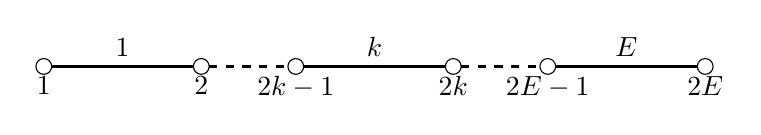
\begin{tikzpicture}
  \draw (2.3,0) circle (0.1) node [below] {$1$};
  \draw (4.3,0) circle (0.1) node [below] {$2$};
  \draw[thick] (2.4,0) -- (4.2,0) node [above,midway] {$1$};
  \draw[thick,dashed] (4.4,0) -- (5.4,0);
  \draw (5.5,0) circle (0.1) node [below] {$2k-1$};
  \draw (7.5,0) circle (0.1) node [below] {$2k$};
  \draw[thick] (5.6,0) -- (7.4,0) node [above,midway] {$k$};
  \draw[thick,dashed] (7.6,0) -- (8.6,0);
  \draw (8.7,0) circle (0.1) node [below] {$2E-1$};
  \draw (10.7,0) circle (0.1) node [below] {$2E$};
  \draw[thick] (8.8,0) -- (10.6,0) node [above,midway] {$E$};
\end{tikzpicture}

  \caption{One-dimensional mesh made of $E$ elements of constant length $\Delta X = \frac{l}{E}$.}\label{fig:1Dmesh}
\end{figure}

Since fields are carried by particles, we seek for the scheme equation that gives the solution $\bar{q}$ at a material point for a given time step, with respect to the solutions of other particles at previous time step. In this section, Latin and Greek symbols are respectively devoted to nodes and material points. Furthermore, since we consider here scalar quantities, the information on nodes and particles can be written as subscripts without ambiguity. Hence, at the time step $n$, the solution at material point $\alpha$ reads $q^{n}_\alpha$ and it is the same for nodes. Then, the cell containing a given particle $\mu$ will be denoted by $c(\mu)$ so that the nodes interacting with this particle are $2c(\mu)-1$ and $2c(\mu)$. At last, the linear shape functions defined in element $c(\mu)$ are:
\begin{equation}
S_{2c(\mu)-1}(X)= \frac{X^{2c(\mu)} - X}{\Delta X} \qquad S_{2c(\mu)}(X)= \frac{X -X^{2c(\mu)-1}}{\Delta X} \qquad X \in \[X^{2c(\mu)-1},X^{2c(\mu)}\]
\end{equation}
and $S_{i,\mu}$ is the shape function of node $i$ evaluated at the position of the $\alpha$th material point.

\subsubsection*{Scheme equation: Euler time discretization}
The method followed to write the scheme equation is to trace backward the numerical procedure described in section \ref{sec:DGMPM} in order to get an expression of the form \eqref{eq:general_scheme} for the material point $I$:
\begin{equation}
\bar{Q}^{n+1}_\alpha = H\(\bar{Q}^{n}_\beta\) \qquad  \beta=1,..,N_p
\end{equation} 
Quantities at time $t^{n+1}$ are obtained by interpolating nodal solutions of the discrete equation \eqref{eq:DGMPM_discrete} in the cell containing the $\alpha$th particle by the projection \eqref{eq:DGMPM_node2points}: 
\begin{equation}
\bar{Q}^{n+1}_\alpha = S_{2c(\alpha)-1,\alpha}\bar{q}_{2c(\alpha)-1}^{n+1} + S_{2c(\alpha),\alpha}\bar{q}_{2c(\alpha)}^{n+1} \label{eq:updated_MP}
\end{equation}
With the interface fluxes in the case of the linear scalar advection equation $\Fc_N =  (aq^*) N $, in which $q^*$ is the stationary solution of Riemann's problem at the cell interface and $N=\pm 1$ the outward unit normal, the discrete form \eqref{eq:DGMPM_discrete} leads to the following expressions of updated nodal values:
\begin{equation}
  \label{eq:nodal_discrete_forms}
  \begin{aligned}
    & \bar{q}_{2c(\alpha)-1}^{n+1}= \bar{q}_{2c(\alpha)-1}^{n} + \frac{\Delta t}{M^L_{2c(\alpha)-1}}\( K_{2c(\alpha)-1,j} a\bar{q}_{j}^{n}- a\rho \bar{q}_{2c(\alpha)-1}^*N_{2c(\alpha)-1} \)\\
    &\bar{q}_{2c(\alpha)}^{n+1}= \bar{q}_{2c(\alpha)}^{n} + \frac{\Delta t}{M^L_{2c(\alpha)}}\( K_{2c(\alpha),j} a\bar{q}_{j}^{n}- a\rho \bar{q}_{2c(\alpha)}^*N_{2c(\alpha)} \)
  \end{aligned}
\end{equation}
Where in a one-dimensional grid, the outward unit vectors are $N_{2c(\alpha)-1}=-1$ and $N_{2c(\alpha)}=1$.

First, the mass density is defined in a cell as the ratio of total nodal mass and the element volume:
\begin{equation}
  \label{eq:grid_density}
  \rho(X) = \frac{M^L_{2c-1}+M^L_{2c}}{\Delta X} = \frac{\sum_{\mu=1}^{N_p^c} m_\mu}{\Delta X}, \qquad X \in [X^{2c-1},X^{2c}]
\end{equation}
where $N_p^{c}$ is the number of particles in cell $c$ and $m_\mu$, the mass carried by the $\mu$th material point. For homogenous medium, we assume the mass is uniformly distributed between patricles so that the previous definition reduces to $\rho = N_p^{c} m^c/\Delta X$, with $m^c$ the mass carried by particles lying in $c$. Then, provided linear shape functions, the lumped mass and the pseudo-stiffness matrices are:
\begin{align}
  & M^L_i = \sum_{\mu=1}^{N_p} S_{i\mu} m_\mu = m^{c(i)} \sum_{\mu=1}^{N_p} S_{i\mu}\\
  & K_{2c(\alpha)-1,j} = \sum_{\mu=1}^{N_p} \drond{S_{2c(\alpha)-1,\mu}}{X} m_\mu S_{j\mu} = -m^{c(i)} \sum_{\mu=1}^{N_p} \frac{ S_{j\mu}}{\Delta X} \\
  & K_{2c(\alpha),j} = \sum_{\mu=1}^{N_p} \drond{S_{2c(\alpha),\mu}}{X} m_\mu S_{j\mu} = m^{c(i)}\sum_{\mu=1}^{N_p} \frac{ S_{j\mu}}{\Delta X} 
\end{align}
The discontinuous approximation basis moreover yields a bloc diagonal pseudo-stiffness matrix so that one can write:
\begin{equation}
  \label{eq:block_diag_K}
  K_{ij} \bar{q}_{j}^{n}= K_{i,2c(i)-1} \bar{q}_{2c(i)-1}^{n}+K_{i,2c(i)} \bar{q}_{2c(i)}^{n}
\end{equation}

A right-going wave (\textit{i.e. $a>0$}) leads to a stationary solution of Riemann problems equals to the state of the upwind node of an interface, that is:
\begin{align}
  & q_{2c(\alpha)-1}^* = \rho \bar{q}^n_{2c(\alpha)-2}=  N_p^{c(\alpha)}\frac{ m^{c(\alpha)}}{\Delta X}\bar{q}^n_{2c(\alpha)-2} \\
  & q_{2c(\alpha)}^* = \rho \bar{q}^n_{2c(\alpha)} =  N_p^{c(\alpha)}\frac{ m^{c(\alpha)}}{\Delta X} \bar{q}^n_{2c(\alpha)} 
\end{align}

Gathering all the previous consideration and seeing that the definition of the mass density used implies that every particles in a given cell carry the same mass, equations \eqref{eq:nodal_discrete_forms} read:
% \begin{equation}
%   \label{eq:nodal_euler}
%   \begin{aligned}
%     & \bar{q}_{2c(\alpha)-1}^{n+1}= \bar{q}_{2c(\alpha)-1}^{n} - \frac{a\Delta t}{\Delta X}\( \frac{m^{c(\alpha)} f_{c(\alpha)}^{n} - N_p^{c( \alpha)}m^{c(\alpha)} \bar{q}^n_{2c(\alpha)-2}}{\sum_{\mu=1}^{N_p^{c(\alpha)}} m^{c(\alpha)} S_{2c(\alpha)-1,\mu}}\)\\
%     &\bar{q}_{2c(\alpha)}^{n+1}= \bar{q}_{2c(\alpha)}^{n} + \frac{a\Delta t}{\Delta X}\( \frac{m^{c(\alpha)}f_{c(\alpha)}^{n}- N_p^{c( \alpha)} m^{c(\alpha)} \bar{q}^n_{2c(\alpha)}}{\sum_{\mu=1}^{N_p^{c(\alpha)}} m^{c(\alpha)} S_{2c(\alpha),\mu}} \)
%   \end{aligned}
% \end{equation
\begin{equation}
  \label{eq:nodal_euler}
  \begin{aligned}
    & \bar{q}_{2c(\alpha)-1}^{n+1}= \bar{q}_{2c(\alpha)-1}^{n} - \frac{a\Delta t}{\Delta X}\( \frac{\sum_{\mu=1}^{N_p^{c(\alpha)}} \[S_{2c(\alpha)-1,\mu}\bar{q}_{2c(\alpha)-1}^{n}+ S_{2c(\alpha),\mu}\bar{q}_{2c(\alpha)}^{n}\] - N_p^{c( \alpha)} \bar{q}^n_{2c(\alpha)-2}}{\sum_{\mu=1}^{N_p^{c(\alpha)}}S_{2c(\alpha)-1,\mu}}\)\\
    &\bar{q}_{2c(\alpha)}^{n+1}= \bar{q}_{2c(\alpha)}^{n} + \frac{a\Delta t}{\Delta X}\( \frac{\sum_{\mu=1}^{N_p^{c(\alpha)}} \[S_{2c(\alpha)-1,\mu}\bar{q}_{2c(\alpha)-1}^{n}+ S_{2c(\alpha),\mu}\bar{q}_{2c(\alpha)}^{n}\]- N_p^{c( \alpha)} \bar{q}^n_{2c(\alpha)}}{\sum_{\mu=1}^{N_p^{c(\alpha)}} S_{2c(\alpha),\mu}} \)
  \end{aligned}
\end{equation}
where the volume fluxes contributions $\sum_{\mu=1}^{N_p^{c}} \[S_{2c-1,\mu}\bar{q}_{2c-1}^{n}+ S_{2c,\mu}\bar{q}_{2c}^{n}\]$ are written for simplicity $f_{c}^{n}$. Note also that the Courant number $a\Delta t/\Delta X$ arises. Introduction of those equation in the updated material point solution \eqref{eq:updated_MP} leads after some simplifications to:
\begin{equation}
  \label{eq:euler_before_mapping}
  \begin{split}
    \bar{Q}^{n+1}_\alpha = S_{2c(\alpha)-1,\alpha}q^n_{2c(\alpha)-1}  &+ S_{2c(\alpha),\alpha}\(1-\frac{a\Delta t}{\Delta X}\frac{N_p^{c(\alpha)}}{\sum_\mu S_{2c(\alpha),\mu}}\)q^n_{2c(\alpha)} +N_p^{c(\alpha)}\frac{a\Delta t}{\Delta X} \frac{S_{2c(\alpha)-1,\alpha}}{\sum_\mu S_{2c(\alpha)-1,\mu}}q^n_{2c(\alpha)-2} \\
    & + \frac{a\Delta t}{\Delta X}\(\frac{S_{2c(\alpha),\alpha}}{\sum_\mu S_{2c(\alpha),\mu}}-\frac{S_{2c(\alpha)-1,\alpha}}{\sum_\mu S_{2c(\alpha)-1,\mu}}\)f_{c(\alpha)}^{n}
  \end{split}
\end{equation}
In equation \eqref{eq:euler_before_mapping} the solutions at nodes result from the convection step \eqref{eq:DGMPM_points2nodes}:
\begin{equation}
\bar{q}^{n}_{i} = \frac{\sum_\beta S_{i\beta}m_\beta \bar{Q}^n_{\beta}}{\sum_\gamma S_{i\gamma}m_\gamma} = \frac{\sum_\beta S_{i\beta} \bar{q}^n_{\beta}}{\sum_\beta S_{i\beta}} \label{eq:stab_mapping}
\end{equation}
In particular, the volume fluxes contributions can be written:
\begin{equation}
  f_{c}^{n}=\sum_{\mu=1}^{N_p^{c}}\[S_{2c-1,\mu}\frac{\sum_\beta S_{2c-1,\beta}\bar{q}^n_{\beta}}{\sum_\mu S_{2c-1,\mu}}+ S_{2c,\mu}\frac{\sum_\beta S_{2c,\beta} \bar{q}^n_{\beta}}{\sum_\mu S_{2c(\mu),\mu}} \]=\sum^{N_p}_{\beta=1}\(S_{2c-1,\beta} +S_{2c,\beta} \)\bar{q}^n_{\beta} \label{eq:volume_fluxes_mapped}
\end{equation}
Thus, introduction of mappings \eqref{eq:stab_mapping} and \eqref{eq:volume_fluxes_mapped} in equation \eqref{eq:euler_before_mapping} and permutation of sums over $\beta$ and $i$ lead after some simplifications to the scheme equation:
\begin{equation}
  \begin{split}
    \bar{Q}^{n+1}_\alpha = \sum_{\beta=1}^{N_p} \bar{Q}^{n}_\beta & \left\lbrace \vphantom{\frac{S_{2c(\alpha)-1,\beta}}{\sum_\mu S_{2c(\alpha)-1,\mu}}}S_{2c(\alpha)-1,\alpha}\frac{S_{2c(\alpha)-1,\beta}}{\sum_\mu S_{2c(\alpha)-1,\mu}} + S_{2c(\alpha),\alpha}\frac{S_{2c(\alpha),\beta}}{\sum_\mu S_{2c(\alpha),\mu}} \right. \\
    & -\frac{a\Delta t}{\Delta X}N_p^{c(\alpha)}\frac{S_{2c(\alpha),\alpha}}{\sum_\mu S_{2c(\alpha),\mu}}\frac{S_{2c(\alpha),\beta}}{\sum_\mu S_{2c(\alpha),\mu}}\\
    & + \frac{a\Delta t}{\Delta X}N_p^{c(\alpha)} \frac{S_{2c(\alpha)-1,\alpha}}{\sum_\mu S_{2c(\alpha)-1,\mu}}\frac{S_{2c(\alpha)-2,\beta}}{\sum_\mu S_{2c(\alpha)-2,\mu}} \\
    &\left.+ \frac{a\Delta t}{\Delta X}\[\frac{S_{2c(\alpha),\alpha}}{\sum_\mu S_{2c(\alpha),\mu}}-\frac{S_{2c(\alpha)-1,\alpha}}{\sum_\mu S_{2c(\alpha)-1,\mu}}\]\(S_{2c(\alpha)-1,\beta} +S_{2c(\alpha),\beta}\) \right\rbrace \label{eq:scheme_euler1}
  \end{split}
\end{equation}
Note that the last term of formula \eqref{eq:scheme_euler1} is non-zero if particles $\beta$ and $\alpha$ share the same cell, and in that case the parenthesis is one. Hence, the scheme equation can be rewritten as:
\begin{equation}
  \label{eq:Euler_scheme}
  \begin{split}
    \bar{Q}^{n+1}_\alpha = \sum_{\beta=1}^{N_p} \bar{Q}^{n}_\beta  &\left\lbrace\sum_{i=1}^{2E}S_{i\beta}\frac{S_{i\alpha}}{\sum_\mu S_{i\mu}}  + N_p^{c(\alpha)}\frac{a\Delta t}{\Delta X} \[\frac{S_{2c(\alpha)-1,\alpha}}{\sum_{\mu}  S_{2c(\alpha)-1,\mu}}\frac{S_{2c(\alpha)-2,\beta}}{\sum_{\mu}  S_{2c(\alpha)-2,\mu}}-\frac{S_{2c(\alpha),\alpha}S_{2c(\alpha),\beta}}{\(\sum_{\mu}  S_{2c(\alpha),\mu}\)^2}\]\right.\\
    & + \left.   \frac{a\Delta t}{\Delta X} \[\frac{S_{2c(\beta),\alpha}}{\sum_{\mu}  S_{2c(\beta),\mu}}-\frac{S_{2c(\beta)-1,\alpha}}{\sum_\mu S_{2c(\beta)-1,\mu}}\] \vphantom{\sum_{i=1}^{2E}}\right\rbrace
  \end{split}
\end{equation}
The first (\textit{resp. second}) brackets in equation \eqref{eq:Euler_scheme} involve shape functions that are non zero if material point $\beta$ and $\alpha$ lie in adjacent cells (\textit{resp. the same cell}). Hence, the numerical domain of dependence of the DGMPM for scalar linear advection with covers two cells regardless of the number of material points. It is worth noticing that in the particular case of one material point lying in every cells, convective phase \eqref{eq:stab_mapping} simplifies to: $\bar{q}^n_i = \bar{Q}^n_\alpha$ for $c(i)=c(\alpha)$. The mapping hence amounts to a piece-wise constant reconstruction of the field on the background grid that makes the DGMPM equivalent to the \textit{First Order Upwind (FOU)} method.
% Moreover, the particular case of one material point lying in every cell leads to the simplified form: 
% \begin{equation}
%   \begin{split}
%     \label{eq:Godunov}
%     \bar{Q}^{n+1}_\alpha = \bar{Q}^{n}_\alpha\(1-\frac{a\Delta t}{\Delta X}\) +\frac{a\Delta t}{\Delta X} \bar{Q}^{n}_{\alpha-1} 
%   \end{split}
% \end{equation}
% which corresponds to the Godunov scheme. This result is due to the convective phase from particles to nodes \eqref{eq:DGMPM_points2nodes} which in the case of a one particle-per-cell discretization leads to a piecewise constant reconstruction of fields on the grid.
However, this no longer holds for other distributions of material points within the computational grid. 

\subsubsection*{Scheme equation: RK2 time discretization}

The solution of the discrete system on the grid for the second-order Runge-Kutta time integration consists in the two-stages procedure \eqref{eq:DGMPM_discrete_RK2} which, particularizes at node $i$ for the one-dimensional scalar linear advection equation as:
\begin{subequations}
  \begin{alignat}{1}
    \label{eq:RK2_stage1}& \bar{q}^{n+1/2}_{i}  =\bar{q}^{n}_{i} + \frac{1}{2}\frac{\Delta t}{M^L_{i}} a \( \sum_{j=1}^{2E} K_{i,j} \bar{q}^n_{j} - q^{*,n}_{i}N_i \) \quad \text{(no sum on $i$)} \\
    \label{eq:RK2_stage2}& \bar{q}^{n+1}_{i}  =\bar{q}^{n}_{i} + \frac{\Delta t}{M^L_{i}} a \( \sum_{j=1}^{2E} K_{i,j} \bar{q}^{n+1/2}_{j} - q^{*,n+1/2}_{i}N_i \) \quad \text{(no sum on $i$)}
  \end{alignat}
\end{subequations}
This procedure can be seen as a recursive use of the Euler scheme \eqref{eq:nodal_euler} with suitable time step sizes. Indeed, the first stage \eqref{eq:RK2_stage1} yields the intermediate nodal fields in cell $c(\alpha)$:
\begin{equation}
  \label{eq:discrete_RK2_step1}
  \begin{aligned}
    &\bar{q}_{2c(\alpha)-1}^{n+1/2}= \bar{q}_{2c(\alpha)-1}^{n} - \frac{a\Delta t}{2\Delta X}\( \frac{f_{c(\alpha)}^{n} - N_p^{c( \alpha)} \bar{q}^n_{2c(\alpha)-2}}{\sum_{\mu=1}^{N_p^{c(\alpha)}}  S_{2c(\alpha)-1,\mu}}\)\\
    &\bar{q}_{2c(\alpha)}^{n+1/2}= \bar{q}_{2c(\alpha)}^{n} + \frac{a\Delta t}{2\Delta X}\( \frac{f_{c(\alpha)}^{n}- N_p^{c( \alpha)}  \bar{q}^n_{2c(\alpha)}}{\sum_{\mu=1}^{N_p^{c(\alpha)}}  S_{2c(\alpha),\mu}} \)
  \end{aligned}
\end{equation}
In addition, the second stage \eqref{eq:RK2_stage2} leads to the expressions of nodal quantities at the end of the time step:
\begin{equation}
  \label{eq:discrete_RK2_step2}
  \begin{aligned}
    &\bar{q}_{2c(\alpha)-1}^{n+1}= \bar{q}_{2c(\alpha)-1}^{n} - \frac{a\Delta t}{\Delta X}\( \frac{\sum_{\gamma=1}^{N_p^{c(\alpha)}}\[S_{2c(\alpha)-1,\gamma}\bar{q}_{2c(\alpha)-1}^{n+1/2}+ S_{2c(\alpha),\gamma}\bar{q}_{2c(\alpha)}^{n+1/2}\] - N_p^{c( \alpha)} \bar{q}^{n+1/2}_{2c(\alpha)-2}}{\sum_{\mu=1}^{N_p^{c(\alpha)}}  S_{2c(\alpha)-1,\mu}}\)\\
    &\bar{q}_{2c(\alpha)}^{n+1}= \bar{q}_{2c(\alpha)}^{n} + \frac{a\Delta t}{\Delta X}\( \frac{\sum_{\gamma=1}^{N_p^{c(\alpha)}}\[S_{2c(\alpha)-1,\gamma}\bar{q}_{2c(\alpha)-1}^{n+1/2}+ S_{2c(\alpha),\gamma}\bar{q}_{2c(\alpha)}^{n+1/2}\]- N_p^{c( \alpha)}  \bar{q}^{n+1/2}_{2c(\alpha)}}{\sum_{\mu=1}^{N_p^{c(\alpha)}}  S_{2c(\alpha),\mu}} \)
  \end{aligned}
\end{equation}
Then, combination of the interpolation from nodes to particles \eqref{eq:updated_MP} and equations \eqref{eq:discrete_RK2_step2} leads, after some simplifications, to the solution at material point $\alpha$ and time step $n+1$:
\begin{equation}
  \begin{split}
    \bar{Q}^{n+1}_\alpha =  &S_{2c(\alpha)-1,\alpha}\bar{q}_{2c(\alpha)-1}^{n} - \(\frac{a\Delta t}{\Delta X}\[S_{2c(\alpha)-1,\alpha} - S_{2c(\alpha),\alpha}\frac{\sum_{\gamma} S_{2c(\alpha)-1,\gamma}}{\sum_{\mu}  S_{2c(\alpha),\mu}}\] \)\bar{q}_{2c(\alpha)-1}^{n+1/2} \\ & +S_{2c(\alpha),\alpha}\bar{q}_{2c(\alpha)}^{n} + \frac{a\Delta t}{\Delta X}\[S_{2c(\alpha),\alpha} - S_{2c(\alpha)-1,\alpha}\frac{\sum_{\gamma} S_{2c(\alpha),\gamma}}{\sum_{\mu}  S_{2c(\alpha)-1,\mu}}- N_p^{c(\alpha)}\frac{S_{2c(\alpha),\alpha}}{\sum_{\mu}  S_{2c(\alpha),\mu}}\] \bar{q}_{2c(\alpha)}^{n+1/2}\\
    &+N_p^{c(\alpha)}\frac{a\Delta t}{\Delta X}\frac{S_{2c(\alpha)-1,\alpha}}{\sum_{\mu}  S_{2c(\alpha)-1,\mu}}\bar{q}_{2c(\alpha)-2}^{n+1/2}
  \end{split}
\end{equation}
Note that the volume fluxes contributions $f_c^{n}$ are used in equations \eqref{eq:discrete_RK2_step1} and not in \eqref{eq:discrete_RK2_step2}. Indeed, nodal values $q_i^{n+1/2}$ provided by the first stage of RK2 algorithm are substituted in the second one, it is therefore better to make them appear explicitly. It thus comes:
\begin{equation}
  \begin{split}
    \bar{Q}^{n+1}_\alpha &=  S_{2c(\alpha)-1,\alpha}\bar{q}_{2c(\alpha)-1}^{n} +S_{2c(\alpha),\alpha}\bar{q}_{2c(\alpha)}^{n} \\
    &- \frac{a\Delta t}{\Delta X}\[S_{2c(\alpha)-1,\alpha} - S_{2c(\alpha),\alpha}\frac{\sum_{\mu} S_{2c(\alpha)-1,\mu}}{\sum_{\mu}  S_{2c(\alpha),\mu}}\] \(\bar{q}_{2c(\alpha)-1}^{n} - \frac{a\Delta t}{2\Delta X}\( \frac{f_{c(\alpha)}^{n} - N_p^{c( \alpha)} \bar{q}^n_{2c(\alpha)-2}}{\sum_{\mu}  S_{2c(\alpha)-1,\mu}}\)\) \\
    &  + \frac{a\Delta t}{\Delta X}\[S_{2c(\alpha),\alpha}\(1- \frac{N_p^{c(\alpha)}}{\sum_{\mu}  S_{2c(\alpha),\mu}}\) - S_{2c(\alpha)-1,\alpha}\frac{\sum_{\mu} S_{2c(\alpha),\mu}}{\sum_{\mu}  S_{2c(\alpha)-1,\mu}}\] \(\bar{q}_{2c(\alpha)}^{n} + \frac{a\Delta t}{2\Delta X}\( \frac{f_{c(\alpha)}^{n}- N_p^{c( \alpha)}  \bar{q}^n_{2c(\alpha)}}{\sum_{\mu}  S_{2c(\alpha),\mu}} \)\)\\
    &+N_p^{c(\alpha)}\frac{a\Delta t}{\Delta X}\frac{S_{2c(\alpha)-1,\alpha}}{\sum_{\mu}  S_{2c(\alpha)-1,\mu}}\(\bar{q}_{2c(\alpha)-2}^{n} + \frac{a\Delta t}{2\Delta X}\( \frac{f_{c(\alpha)-1}^{n}- N_p^{c( \alpha)}  \bar{q}^n_{2c(\alpha)-2}}{\sum_{\mu}  S_{2c(\alpha)-2,\mu}} \)\) \label{eq:Mp_before_mapping}
  \end{split}
\end{equation}
Note that the second equation of the set \eqref{eq:discrete_RK2_step1} is used for $q^{n+1/2}_{2c(\alpha)-2}$ since it is the downwstream node of the adjacent cell $c(\alpha)-1$. At last, by rearranging formula \eqref{eq:Mp_before_mapping} as:
\begin{equation}
  \begin{split}
    \bar{Q}^{n+1}_\alpha =  &\(S_{2c(\alpha)-1,\alpha} -\frac{a\Delta t}{\Delta X}\[S_{2c(\alpha)-1,\alpha} - S_{2c(\alpha),\alpha}\frac{\sum_{\mu} S_{2c(\alpha)-1,\mu}}{\sum_{\mu}  S_{2c(\alpha),\mu}}\]\)\bar{q}_{2c(\alpha)-1}^{n} \\
    +&\(S_{2c(\alpha),\alpha} + \frac{a\Delta t}{\Delta X}\[S_{2c(\alpha),\alpha}\(1-\frac{N_p^{c(\alpha)}}{\sum_{\mu}  S_{2c(\alpha),\mu}}\) - S_{2c(\alpha)-1,\alpha}\frac{\sum_{\mu} S_{2c(\alpha),\mu}}{\sum_{\mu}  S_{2c(\alpha)-1,\mu}}\]\) \bar{q}_{2c(\alpha)}^{n} \\
    +&\frac{1}{2}\(\frac{a\Delta t}{\Delta X}\)^2\(N_p^{c( \alpha)}\[\frac{S_{2c(\alpha)-1,\alpha}}{\sum_\mu S_{2c(\alpha)-1,\mu}} - \frac{S_{2c(\alpha),\alpha}}{\sum_{\mu}  S_{2c(\alpha),\mu}}\] +S_{2c(\alpha),\alpha} \(\frac{N_p^{c(\alpha)}}{\sum_{\mu}  S_{2c(\alpha),\mu}}\)^2\)\bar{q}_{2c(\alpha)}^{n}\\
    +&N_p^{c( \alpha)}\frac{a\Delta t}{\Delta X}  \[ \frac{S_{2c(\alpha)-1,\alpha}}{\sum_{\mu}  S_{2c(\alpha)-1,\mu}}\(1 -   \frac{a\Delta t}{2\Delta X}\(1+\frac{N_p^{c( \alpha)} }{\sum_{\mu}  S_{2c(\alpha)-2,\mu}} \)\)+\frac{a\Delta t}{2\Delta X} \frac{S_{2c(\alpha),\alpha}}{\sum_{\mu}  S_{2c(\alpha),\mu}}\]\bar{q}^n_{2c(\alpha)-2}\\
    -&\frac{1}{2}\(\frac{a\Delta t}{\Delta X}\)^2 N_p^{c(\alpha)}\frac{S_{2c(\alpha),\alpha}}{\(\sum_{\mu}  S_{2c(\alpha),\mu}\)^2} f_{c(\alpha)}^{n} +\frac{1}{2}\(\frac{a\Delta t}{\Delta X}\)^2N_p^{c(\alpha)}\frac{S_{2c(\alpha)-1,\alpha}}{\sum_{\mu}  S_{2c(\alpha)-1,\mu}}\frac{ f_{c(\alpha)-1}^{n}}{\sum_{\mu}  S_{2c(\alpha)-2,\mu}}
  \end{split}
\end{equation}
the use of convective phase equations \eqref{eq:stab_mapping} and \eqref{eq:volume_fluxes_mapped} allows to write:
\begin{equation}
  \begin{split}
    \bar{Q}^{n+1}_\alpha =  &\sum_{\beta} \bar{Q}_\beta^n  \left\lbrace \frac{S_{2c(\alpha)-1,\beta}}{\sum_\mu S_{2c(\alpha)-1,\mu}}\(S_{2c(\alpha)-1,\alpha} -\frac{a\Delta t}{\Delta X}\[S_{2c(\alpha)-1,\alpha} - S_{2c(\alpha),\alpha}\frac{\sum_{\gamma} S_{2c(\alpha)-1,\gamma}}{\sum_{\mu}  S_{2c(\alpha),\mu}}\]\)  \right. \\
    &+\frac{S_{2c(\alpha),\beta}}{\sum_\mu S_{2c(\alpha),\mu}}\(S_{2c(\alpha),\alpha} + \frac{a\Delta t}{\Delta X}\[S_{2c(\alpha),\alpha}\(1-\frac{N_p^{c(\alpha)}}{\sum_{\mu}  S_{2c(\alpha),\mu}}\) - S_{2c(\alpha)-1,\alpha}\frac{\sum_{\gamma} S_{2c(\alpha),\gamma}}{\sum_{\mu}  S_{2c(\alpha)-1,\mu}}\]\)  \\
    &+\frac{S_{2c(\alpha),\beta}}{\sum_\mu S_{2c(\alpha),\mu}}\frac{1}{2}\(\frac{a\Delta t}{\Delta X}\)^2\(N_p^{c( \alpha)}\[\frac{S_{2c(\alpha)-1,\alpha}}{\sum_\mu S_{2c(\alpha)-1,\mu}} - \frac{S_{2c(\alpha),\alpha}}{\sum_{\mu}  S_{2c(\alpha),\mu}}\] +S_{2c(\alpha),\alpha} \(\frac{N_p^{c(\alpha)}}{\sum_{\mu}  S_{2c(\alpha),\mu}}\)^2\)  \\
    &+\frac{N_p^{c( \alpha)} S_{2c(\alpha)-2,\beta}}{\sum_\mu S_{2c(\alpha)-2,\mu}}\frac{a\Delta t}{\Delta X} \[ \frac{S_{2c(\alpha)-1,\alpha}}{\sum_{\mu}  S_{2c(\alpha)-1,\mu}}\(1 -   \frac{a\Delta t}{2\Delta X}\(1+\frac{N_p^{c( \alpha)} }{\sum_{\mu}  S_{2c(\alpha)-2,\mu}} \)\)+\frac{a\Delta t}{2\Delta X} \frac{S_{2c(\alpha),\alpha}}{\sum_{\mu}  S_{2c(\alpha),\mu}}\]\\
    &+\frac{1}{2}\(\frac{a\Delta t}{\Delta X}\)^2 N_p^{c(\alpha)}\left.\( \frac{\[S_{2c(\alpha)-2,\beta} +S_{2c(\alpha)-3,\beta} \]}{\sum_{\mu}  S_{2c(\alpha)-1,\mu}\sum_{\mu}  S_{2c(\alpha)-2,\mu}} S_{2c(\alpha)-1,\alpha}-\frac{\[S_{2c(\alpha)-1,\beta} +S_{2c(\alpha),\beta} \]}{\(\sum_{\mu}  S_{2c(\alpha),\mu}\)^2} S_{2c(\alpha),\alpha}\)  \right\rbrace
  \end{split}
\end{equation}
Once the previous formula is simplified, the one-dimensional scheme equation of the DGMPM with the RK2 time discretization can be written as:
\begin{equation}
  \label{eq:RK2_scheme}
  \begin{split}
    \bar{Q}^{n+1}_\alpha =  &\sum_{\beta} \bar{Q}_\beta^n  \left\lbrace \sum_i S_{i\beta}\frac{S_{i\alpha}}{\sum_\mu S_{i\mu}}
      +\frac{a\Delta t}{\Delta X}\[\frac{S_{2c(\beta),\alpha}}{\sum_{\mu}  S_{2c(\beta),\mu}} - \frac{S_{2c(\beta)-1,\alpha}}{\sum_{\mu}  S_{2c(\beta)-1,\mu}}\] \right.\\
    &+\frac{a\Delta t}{\Delta X}N_p^{c( \alpha)}\[\frac{S_{2c(\alpha)-1,\alpha}}{\sum_{\mu}  S_{2c(\alpha)-1,\mu}}\frac{S_{2c(\alpha)-2,\beta}}{\sum_\mu S_{2c(\alpha)-2,\mu}}-\frac{S_{2c(\alpha),\alpha}S_{2c(\alpha),\beta}}{\(\sum_\mu S_{2c(\alpha),\mu}\)^2}\] \\
    &+\frac{1}{2}\(\frac{a\Delta t}{\Delta X}\)^2N_p^{c( \alpha)} \(\frac{S_{2c(\alpha),\beta}}{\sum_\mu S_{2c(\alpha),\mu}}-\frac{S_{2c(\alpha)-2,\beta}}{\sum_\mu S_{2c(\alpha)-2,\mu}}\)\[\frac{S_{2c(\alpha)-1,\alpha}}{\sum_\mu S_{2c(\alpha)-1,\mu}} - \frac{S_{2c(\alpha),\alpha}}{\sum_{\mu}  S_{2c(\alpha),\mu}}\]\\
    &+\frac{1}{2}\(\frac{a\Delta t}{\Delta X}\)^2N_p^{c( \alpha)}\frac{S_{2c(\beta),\alpha}}{\(\sum_{\mu}  S_{2c(\alpha),\mu}\)^2} \[N_p^{c( \alpha)}\frac{S_{2c(\alpha),\beta} }{\sum_\mu S_{2c(\alpha),\mu}}-1\]\\
    &+ \frac{1}{2}\(\frac{a\Delta t}{\Delta X}\)^2\frac{S_{2c(\beta)+1,\alpha}N_p^{c(\alpha)}}{\sum_{\mu}  S_{2c(\alpha)-1,\mu}\sum_{\mu}  S_{2c(\alpha)-2,\mu}} \left.\[ 1 - N_p^{c( \alpha)}\frac{S_{2c(\alpha)-2,\beta} }{\sum_{\mu}  S_{2c(\alpha)-2,\mu}}\] \right\rbrace
    \end{split}
\end{equation}
The first braces of the latter scheme equation correspond to that obtained for the Euler algorithm \eqref{eq:Euler_scheme} while the second order terms are provided by the two-stages time integration. The brackets in those higher order corrections vanish when only one point is in each cell of the grid, so that the scheme is, as that of the previous section, equivalent to the FOU method.

\subsubsection*{The von Neumann linear stability analysis}
The scheme equations obtained above are written for simplicity:
\begin{equation}
\bar{Q}^{n+1}_\alpha = \sum_{\beta=1}^{N_p} \bar{Q}^n_{\beta} D_{\alpha\beta} \label{eq:scheme_Dpi}
\end{equation}
Moreover, the computational domain is repeated periodically by mapping it to the domain $[-l,0]$ so that the solution at material point $I$ and time step $n$ is expanded into a discrete Fourier basis of $2E+1$ harmonics over the domain $X \in \[-l,l\]$:
\begin{equation}
\bar{Q}^{n}_\alpha = \sum_{j=-E}^{E}A_j^n e^{i \alpha k_j \Delta X}
\end{equation}
with $A^n_j$, the magnitude of the $j$th harmonic at time step $n$, $i = \sqrt{-1}$, and $k_j$ a wave number. Introduction of this expansion in equation \eqref{eq:scheme_Dpi} yields:
\begin{equation}
A_j^{n+1} e^{i\alpha k_j \Delta X} = \sum_{\beta=1}^{N_p} A_j^n D_{\alpha\beta}e^{i \beta k_j \Delta X}\quad \forall j=-E,...,E
\end{equation}
The amplification factor between two time steps at a given point is defined as:
\begin{equation}
\frac{A_j^{n+1}}{A_j^n} = \sum_{\beta=1}^{N_p} e^{i (\beta -\alpha)k_j \Delta X} D_{\alpha\beta} \quad \forall j=-E,...,E \label{eq:fourier_expansion}
\end{equation}
A necessary condition to ensure the stability of a numerical scheme is that the amplification factor must be lower than one in modulus: $\abs{A^{n+1}/A^n} < 1$. This upper bound allows to ensure that eventual errors do not increase during the computation. For expression \eqref{eq:fourier_expansion}, this leads to:
\begin{equation}
 \abs{\sum_{\beta=1}^{N_p} e^{i (\beta -\alpha)k_j \Delta X} D_{\alpha\beta}} \leq \sum_{\beta=1}^{N_p} \abs{e^{i (\beta -\alpha)k_j \Delta X} D_{\alpha\beta}} = \sum_{\beta=1}^{N_p} \abs{D_{\alpha\beta}}
\end{equation}
where the triangle inequality, and the unit modulus of the complex number $e^{\alpha (\beta -\alpha)k_j \Delta X}$ have been used.
Hence, the DGMPM scheme is stable for a given discretization if the Courant number is set so that the following condition is satisfied for all material points:
\begin{equation}
  \label{eq:stability} \sum_{\beta=1}^{N_p} \abs{D_{\alpha\beta}} \leq 1 \quad \forall \: I = 1,...,N_p
\end{equation}
Hence, the stability of the scheme is ensured by using the lowest CFL number resulting from the solution of \eqref{eq:stability} for every material points. According to scheme equations \eqref{eq:Euler_scheme} or \eqref{eq:RK2_scheme}, such a stability condition can be very hard to deal with analytically for general discretizations. 
\begin{table}[h]
  \centering
  \begin{tabular}[ht]{cccccN}
  \hline
  \multicolumn{2}{c}{Number of particles} & Position of $I$th particle in cell $c$ & Euler CFL & RK2 CFL &\\[6pt]
  \hline
  \hline
  (--) &1 &$X^1 \in \[X^{2c-1},X^{2c}\]$  &  1 & 1&\\[8pt]
  \hline
  (i)& 2 & $ X^I= X^{2c-1}+(2I-1)\frac{\Delta X}{4}$ &  0.43 & 1&\\[8pt]
  (ii)& 2 & $X^I= X^{2c-1}+(2I-1)\frac{\Delta X}{4} +\frac{\Delta X}{10} $ &  0.40 & 0.50 &\\[8pt]
  (iii)& 2 & $X^I= X^{2c-1}+(2I-1)\frac{\Delta X}{4} +(I-2)\frac{\Delta X}{10} $ &  0.27 & 1 &\\[8pt]
  (iii)'& 2 & $X^I= X^{2c-1}+(2I-1)\frac{\Delta X}{4} +(I-2)\frac{\Delta X}{4} $ &  0 & 1 &\\[8pt]
  \hline
  (i)& 3 & $ X^I= X^{2c-1}+2I\frac{\Delta X}{8}$ &  0.43 & 1&\\[8pt]
  (ii)& 3 & $X^I= X^{2c-1}+2I\frac{\Delta X}{8} +\frac{\Delta X}{10} $ &  0.40 & 0.50 &\\[8pt]
  (iii)& 3 & $X^I= X^{2c-1}+2I\frac{\Delta X}{8} +(I-2)\frac{\Delta X}{10} $ &  0.27 & 1 &\\[8pt]
  (iii)'& 3 & $X^I= X^{2c-1}+2I\frac{\Delta X}{8} +(I-2)\frac{\Delta X}{4} $ &  0 & 1 &\\[8pt]
  \hline
  (i)& 4 & $ X^I= X^{2c-1}+I\frac{\Delta X}{5}$ &  0.35 & 1&\\[8pt]
  (ii)& 4 & $X^I= X^{2c-1}+I\frac{\Delta X}{5} +\frac{\Delta X}{10} $ &  0.31 & 0.40 &\\[8pt]
  (iii)& 4 & $X^I= X^{2c-1}+I\frac{\Delta X}{5} +\frac{2I-5}{\abs{2I-5}}\frac{\Delta X}{10} $ &  0.18 & 1 &\\[8pt]
  (iii)'& 4 & $X^I= X^{2c-1}+I\frac{\Delta X}{5} +\frac{2I-5}{\abs{2I-5}}\frac{\Delta X}{5} $ &  0 & 1 &\\[8pt]
  \hline
\end{tabular}

%%% Local Variables: 
%%% mode: latex
%%% TeX-master: "../../mainManuscript"
%%% End:
  \caption{DGMPM critical Courant numbers values for Euler or RK2 time integration with respect of the number and positions of material points in a one-dimensional grid. Black circles denote material points while white ones represent grid nodes.}
  \label{tab:CFL_comparison}
\end{table}
Although the infinity of possible material points distributions prevents the explicit derivation of a general stability condition, the optimal CFL number satisfying the equality in equation \eqref{eq:stability} can be find numerically. Some configurations are studied in table \ref{tab:CFL_comparison} and the critical Courant number resulting from the two time discretizations studied above are compared for each. Those results have been obtained by assuming that the particle distribution is the same in every element of a one-dimensional regular mesh so that a material point $\alpha$ must lie between the nodes of the cell it belongs to, that is, $X^I \in \[X^{2c-1},X^{2c}\]$. First, the DGMPM scheme is stable for all CFL number lower to or equal one when cells contain one particle only regardless of their Positions. Then, when many material points share the same element, several configurations are considered:
\begin{itemize}
\item[(i)] particles are positioned symmetrically with respect to cells centers and regularly spaced in the mesh. This space discretization is referred to as the natural configuration in the following.
\item[(ii)] particles initially symmetrically positioned are shifted of $u=\Delta X/10$ with respect to cells centers and regularly spaced in the mesh.
\item[(iii)] the same than (ii) with $u$ so that the first material point overlaps the left node.
\item[(iv)] the same than (ii) with $u$ so that the last material point overlaps the right node.
\item[(v)] particles are placed symmetrically with respect to cells centers but not regularly spaced in the mesh.
\item[(vi)] the same than (v) with the first and last particles overlapping left and right nodes of cells respectively.
\end{itemize}
RK2 results bad when the upwind material point move to the right
One can see in table \ref{tab:CFL_comparison} that the RK2 time discretization provides better results in terms of CFL number for the distributions of particles considered. However, a uniform translation of material points in the mesh leads to a decrease in the Courant number for both time integrations. Furthermore the impact of such a translation is more significant in the stream direction (\textit{i.e. cases (ii) and (iv)}) in such a way that the decline in CFL number is bigger than for an inverse stream direction (\textit{i.e. cases (iii)}). In the latter situation, the Euler algorithm provides even better results than in the natural configuration. One the other hand, particles distributions that conserve the symmetry with respect to cells centers lead to the optimal stability condition when using the RK2 time integration while the Euler CFL depends on the spacing between material points. More specifically, Euler algorithm leads to a vanishing CFL for the case (vi), thus preventing any simulation. Therefore, the distribution of material points, and hence the resulting quadrature, has an influence on the stability of the scheme. As a consequence, the optimal Courant number can be reached even with the Euler discretization, while the classical DGFEM scheme developed in \cite{Chavent_Salzano} is restricted to condition $\Delta t / \Delta X = \Oc(\sqrt{\Delta X})$. This limitation has been addressed by introducing slope limiters in order to remove non-physical oscillations in the vicinity of sharp solutions while providing high-order accuracy in smooth regions \cite{Chavent_Cockburn}. However, the stability of the method was still bounded by $CFL\leq 1/2$ and the scheme was first-order accurate. The use of a second-order Runge kutta \cite{DGFEM_CFL} allowed to achieve second-order accuracy of the scheme, but the stability condition then reduced to $CFL\leq1/3$. More recently, space–time DGFEM formulations \cite{ST_DGFEM1,ST_DGFEM2} provided the ability to relax constraints of pure space DGFEM and obtain a critical CFL at 1.

%%%
The von Neumann linear stability analysis performed in this section provides an explicit (nonlinear) condition \eqref{eq:stability} that must be satisfied in order to ensure the stability of the DGMPM schemes based on both Euler and RK2 time discretizations. First, this relation allows to fully exploit the ability of the method to rebuild the grid mesh arbitrarily. Indeed, after such a procedure, the number and positions of material points in grid cells can change and one must be able to adapt properly the CFL number so that the scheme remains stable. An advantage on the original MPM is hence highlighted since no stability condition exists for the method. Second, it has been shown that some DGMPM discretizations provide an improvement of the restrictive CFL number that applies to the DGFEM scheme. In particular, the optimal condition allowing to capture discontinuities ($CFL=1$) can be reached for several space-time discretizations. This property turns out to be a strength for the DGMPM since it aims at follow waves accurately.

One can imagine to place material points so that an optimal stability condition is reached by minimizing some functional contrained with the description of material boundaries.

\subsection{Convergence analysis of the one-dimensonal scheme}
We now propose to focus on convergence properties in order to define the order accuracy of one-dimensional DGMPM schemes. For the one-dimensonal scalar linear advecton equation with $a>0$, the following theorem holds: 
\begin{theorem}[Roe \cite{Toro}]
  A numerical scheme of the form:
  \begin{equation}
    \label{eq:2}
    q^{n+1}_\alpha=\sum_{\beta=-\infty}^{\infty} D_{\beta} q^{n}_{\alpha+\beta}
  \end{equation}
  is $p$th order accurate ($p\geq 0$) in space and time if and only if
  \begin{equation}
    \label{eq:3}
    \sum_\beta \beta^q D_{\beta} = \(-a\frac{\Delta t}{\Delta X}\)^q \quad 0 \leq q \leq p
  \end{equation}
\end{theorem}
However, the complexity of scheme equations \eqref{eq:Euler_scheme} and \eqref{eq:RK2_scheme} prevent from a straightforward proof of accuracy beyond order zero. As a consequence, the convergence analysis is carried out here numerically unlike the stability analysis. To this end, we still consider the homogeneous one-dimensional medium of the previous section, submitted to an enforced level 

One material point per cell
$\bar{\sigma} \sin\(\frac{4\pi t}{T}\)$
CFL for mpm set to 0.5


\begin{figure}[ht]
  \centering
  {\definecolor{Purple}{RGB}{120,28,129}
\definecolor{Blue}{RGB}{63,96,174}
\definecolor{Duck}{RGB}{83,158,182}
\definecolor{Green}{RGB}{109,179,136}
\definecolor{Yellow}{RGB}{202,184,67}
\definecolor{Orange}{RGB}{231,133,50}
\definecolor{Red}{RGB}{217,33,32}
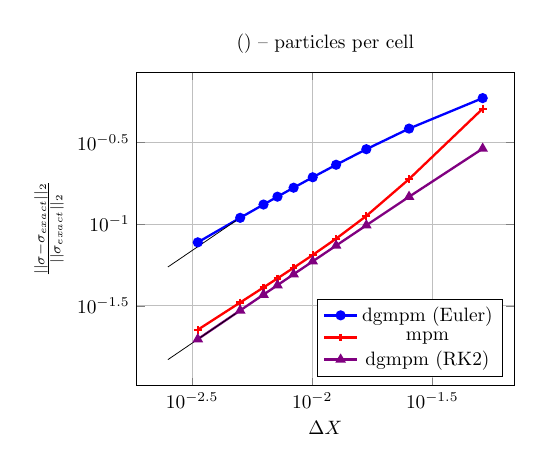
\begin{tikzpicture}[scale=0.7]
\begin{loglogaxis}[xlabel=$\Delta X$,ylabel=$\frac{||\sigma- \sigma_{exact}||_2}{||\sigma_{exact}||_2}$,ymajorgrids=true,xmajorgrids=true,legend pos=south east,title={() -- particles per cell}]
\addplot[Blue,very thick,mark=*] coordinates {(0.05128205128205128,0.5893536686288803) (0.025316455696202535,0.38365050461820954) (0.01680672268907563,0.28694121783258) (0.012578616352201259,0.23042992590093) (0.010050251256281405,0.1932064411839267) (0.008368200836820083,0.166758514421651) (0.007168458781362007,0.1469576790416971) (0.006269592476489028,0.13155393217242628) (0.005012531328320802,0.10909713160359173) (0.00333889816360601,0.07724729297813994) };
\addplot[Red,very thick,mark=+] coordinates {(0.05128205128205128,0.5078512384708146) (0.025316455696202535,0.18826849382667404) (0.01680672268907563,0.1120554030795599) (0.012578616352201259,0.08133103871660345) (0.010050251256281405,0.06462439616740177) (0.008368200836820083,0.053958564987796054) (0.007168458781362007,0.04647624925701119) (0.006269592476489028,0.04089866088480404) (0.005012531328320802,0.0330835719539677) (0.00333889816360601,0.022526233099086298) };
\addplot[Purple,very thick,mark=triangle*] coordinates {(0.05128205128205128,0.2891738981142733) (0.025316455696202535,0.14679510141888402) (0.01680672268907563,0.09821148280234743) (0.012578616352201259,0.07377182111730704) (0.010050251256281405,0.05906759639011608) (0.008368200836820083,0.04924943612717903) (0.007168458781362007,0.042229406220940874) (0.006269592476489028,0.036960694946397976) (0.005012531328320802,0.029579402516102707) (0.00333889816360601,0.019728868588375473) };
\legend{dgmpm (Euler),mpm,dgmpm (RK2)}\addplot[black] coordinates {(0.005012531328320802,0.029579402516102707) (0.002506265664160401,0.014789701258051353)};\addplot[black] coordinates {(0.005012531328320802,0.10909713160359173) (0.002506265664160401,0.054548565801795866)};
\end{loglogaxis}
\end{tikzpicture}
}
  {\definecolor{Purple}{RGB}{120,28,129}
\definecolor{Blue}{RGB}{63,96,174}
\definecolor{Duck}{RGB}{83,158,182}
\definecolor{Green}{RGB}{109,179,136}
\definecolor{Yellow}{RGB}{202,184,67}
\definecolor{Orange}{RGB}{231,133,50}
\definecolor{Red}{RGB}{217,33,32}
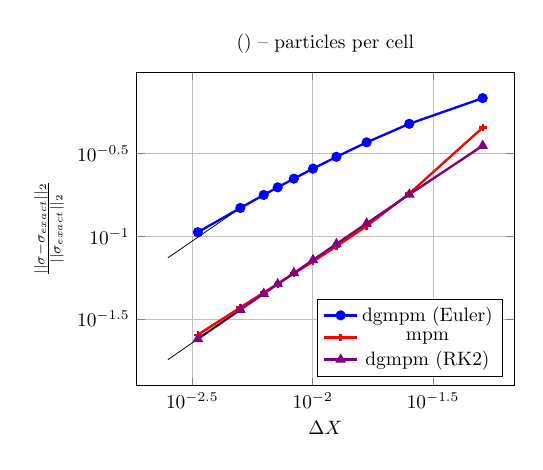
\begin{tikzpicture}[scale=0.7]
\begin{loglogaxis}[xlabel=$\Delta X$,ylabel=$\frac{||\sigma- \sigma_{exact}||_2}{||\sigma_{exact}||_2}$,ymajorgrids=true,xmajorgrids=true,legend pos=south east,title={() -- particles per cell}]
\addplot[Blue,very thick,mark=*] coordinates {(0.05084745762711864,0.68113252282486) (0.025210084033613446,0.476750805595349) (0.01675977653631285,0.368357190488791) (0.012552301255230125,0.30132017517058696) (0.010033444816053514,0.2556619642123912) (0.008356545961002786,0.22249256778190016) (0.007159904534606205,0.19726215089428928) (0.006263048016701462,0.17739888040710228) (0.005008347245409015,0.14807128589226984) (0.003337041156840934,0.10572975254810454) };
\addplot[Red,very thick,mark=+] coordinates {(0.05084745762711864,0.45248984077263216) (0.025210084033613446,0.1808766851772935) (0.01675977653631285,0.11524004898925723) (0.012552301255230125,0.08681586517079888) (0.010033444816053514,0.07040711004025481) (0.008356545961002786,0.05949917036231313) (0.007159904534606205,0.051639746699918304) (0.006263048016701462,0.04567411433926447) (0.005008347245409015,0.037174232059622773) (0.003337041156840934,0.025470523255878463) };
\addplot[Purple,very thick,mark=triangle*] coordinates {(0.05084745762711864,0.3516876642354787) (0.025210084033613446,0.17864402671192) (0.01675977653631285,0.11953909686537742) (0.012552301255230125,0.08979633822041656) (0.010033444816053514,0.07189915852021322) (0.008356545961002786,0.059948366792706105) (0.007159904534606205,0.05140327881277545) (0.006263048016701462,0.04498989825165278) (0.005008347245409015,0.03600491379308246) (0.003337041156840934,0.024014251701450866) };
\legend{dgmpm (Euler),mpm,dgmpm (RK2)}
\addplot[black] coordinates {(0.005008347245409015,0.03600491379308246) (0.0025041736227045075,0.01800245689654123)};\addplot[black] coordinates {(0.005008347245409015,0.14807128589226984) (0.0025041736227045075,0.07403564294613492)};
\end{loglogaxis}
\end{tikzpicture}
}
  {\definecolor{Purple}{RGB}{120,28,129}
\definecolor{Blue}{RGB}{63,96,174}
\definecolor{Duck}{RGB}{83,158,182}
\definecolor{Green}{RGB}{109,179,136}
\definecolor{Yellow}{RGB}{202,184,67}
\definecolor{Orange}{RGB}{231,133,50}
\definecolor{Red}{RGB}{217,33,32}
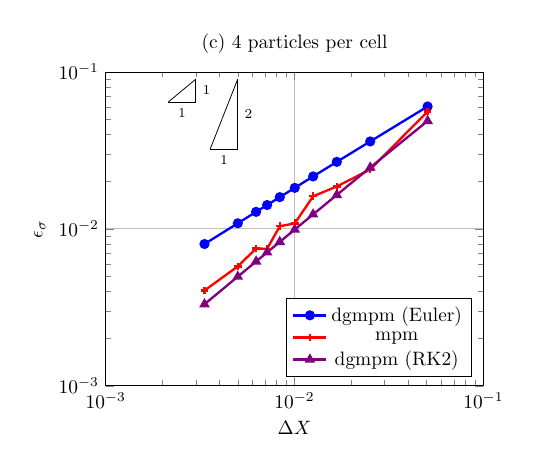
\begin{tikzpicture}[scale=0.7]
\begin{loglogaxis}[xlabel=$\Delta X$,ylabel=$\epsilon_\sigma$,ymajorgrids=true,xmajorgrids=true,legend pos=south east,title={(c) 4 particles per cell},xmin=0.001,xmax=0.1,ymin=0.001,ymax=0.1]
\addplot[Blue,very thick,mark=*] coordinates {(0.05063291139240507,0.06028254805310215) (0.02515723270440252,0.03609159513019716) (0.016736401673640166,0.02673829423087577) (0.012539184952978056,0.021589425529184064) (0.010025062656641603,0.018259587769245567) (0.008350730688935281,0.015933028163219204) (0.007155635062611806,0.014191633450046695) (0.00625978090766823,0.012839170144598252) (0.005006257822277847,0.010858263097309794) (0.003336113427856547,0.008006873276563799) };
\addplot[Red,very thick,mark=+] coordinates {(0.05063291139240507,0.05596279585017391) (0.02515723270440252,0.023927672682306222) (0.016736401673640166,0.0186340535029745) (0.012539184952978056,0.016133897266376464) (0.010025062656641603,0.010844841481788294) (0.008350730688935281,0.010394814959272032) (0.007155635062611806,0.007465947093828996) (0.00625978090766823,0.007505354391812321) (0.005006257822277847,0.005768057197384396) (0.003336113427856547,0.004050678769799506) };
\addplot[Purple,very thick,mark=triangle*] coordinates {(0.05063291139240507,0.048737887930702446) (0.02515723270440252,0.024615842879356833) (0.016736401673640166,0.016465403281250422) (0.012539184952978056,0.01236961744634676) (0.010025062656641603,0.009905565315865) (0.008350730688935281,0.008260121966611404) (0.007155635062611806,0.007083462282011589) (0.00625978090766823,0.006200233048736664) (0.005006257822277847,0.004962654463512573) (0.003336113427856547,0.003310630171855819) };
\legend{dgmpm (Euler),mpm,dgmpm (RK2)}
\draw (axis cs:0.003,0.09) -- (axis cs:0.003/1.4,0.09/1.4);
\draw (axis cs:0.003,0.09) -- (axis cs:0.003,0.09/1.4) node [midway,right] {\scriptsize 1};
\draw (axis cs:0.003,0.09/1.4) -- (axis cs:0.003/1.4,0.09/1.4) node [midway,below] {\scriptsize 1};
\draw (axis cs:0.005,0.09) -- (axis cs:0.005/1.4,0.09/2.8);
\draw (axis cs:0.005,0.09) -- (axis cs:0.005,0.09/2.8) node [midway,right] {\scriptsize 2};
\draw (axis cs:0.005,0.09/2.8) -- (axis cs:0.005/1.4,0.09/2.8) node [midway,below] {\scriptsize 1};
\end{loglogaxis}
\end{tikzpicture}
}
  {\definecolor{Purple}{RGB}{120,28,129}
\definecolor{Blue}{RGB}{63,96,174}
\definecolor{Duck}{RGB}{83,158,182}
\definecolor{Green}{RGB}{109,179,136}
\definecolor{Yellow}{RGB}{202,184,67}
\definecolor{Orange}{RGB}{231,133,50}
\definecolor{Red}{RGB}{217,33,32}
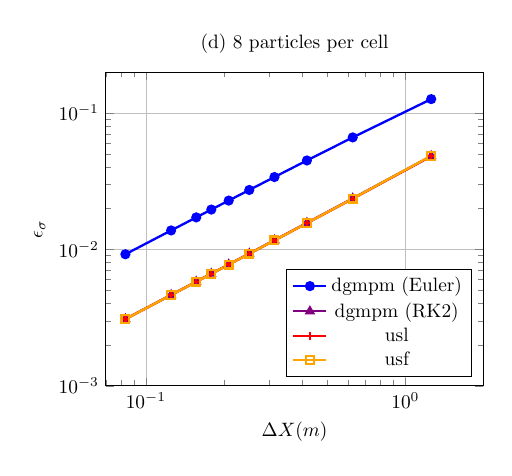
\begin{tikzpicture}[scale=0.7]
\begin{loglogaxis}[xlabel=$\Delta X (m)$,ylabel=$\epsilon_\sigma$,ymajorgrids=true,xmajorgrids=true,legend pos=south east,title={(d) 8 particles per cell},xmin=0.07,xmax=2.,ymin=0.001,ymax=0.2]
\addplot[Blue,very thick,mark=*] coordinates {(1.257861635220126,0.1265027745157943) (0.6269592476489029,0.06627118043883007) (0.4175365344467641,0.04488824642945697) (0.31298904538341155,0.0339372685694115) (0.2503128911138923,0.02728157664595283) (0.20855057351407716,0.02280847579493331) (0.1787310098302055,0.01959561218102149) (0.1563721657544957,0.01717616458221602) (0.12507817385866166,0.013774729917380928) (0.08336807002917881,0.00921347769596086) };
\addplot[Purple,very thick,mark=triangle*] coordinates {(1.257861635220126,0.04835932699145331) (0.6269592476489029,0.023664898920670398) (0.4175365344467641,0.015650087408610885) (0.31298904538341155,0.011688528976777642) (0.2503128911138923,0.00932689601770878) (0.20855057351407716,0.0077589893789605045) (0.1787310098302055,0.006642289744049861) (0.1563721657544957,0.00580654931479797) (0.12507817385866166,0.0046391020056021325) (0.08336807002917881,0.0030872450464644553) };
\addplot[Red,very thick,mark=+] coordinates {(1.257861635220126,0.0482500577228363) (0.6269592476489029,0.023515804312842222) (0.4175365344467641,0.015563635944680462) (0.31298904538341155,0.0116338061608998) (0.2503128911138923,0.009289375524371897) (0.20855057351407716,0.007731700489932084) (0.1787310098302055,0.006621551620111033) (0.1563721657544957,0.005790250848186348) (0.12507817385866166,0.004628260060492159) (0.08336807002917881,0.0030821351983604216) };
\addplot[Orange,very thick,mark=square] coordinates {(1.257861635220126,0.04856012249795517) (0.6269592476489029,0.02358106597523298) (0.4175365344467641,0.015591938841509882) (0.31298904538341155,0.011649502990537916) (0.2503128911138923,0.009299183091519971) (0.20855057351407716,0.007738324260403759) (0.1787310098302055,0.006626289165300689) (0.1563721657544957,0.005793816817189639) (0.12507817385866166,0.00463058418635914) (0.08336807002917881,0.003083476129520196) };
\legend{dgmpm (Euler),dgmpm (RK2),usl,usf}
\draw (axis cs:0.003,0.09) -- (axis cs:0.003/1.4,0.09/1.4);
\draw (axis cs:0.003,0.09) -- (axis cs:0.003,0.09/1.4) node [midway,right] {\scriptsize 1};
\draw (axis cs:0.003,0.09/1.4) -- (axis cs:0.003/1.4,0.09/1.4) node [midway,below] {\scriptsize 1};
\draw (axis cs:0.005,0.09) -- (axis cs:0.005/1.4,0.09/2.8);
\draw (axis cs:0.005,0.09) -- (axis cs:0.005,0.09/2.8) node [midway,right] {\scriptsize 2};
\draw (axis cs:0.005,0.09/2.8) -- (axis cs:0.005/1.4,0.09/2.8) node [midway,below] {\scriptsize 1};
\end{loglogaxis}
\end{tikzpicture}
}
  \caption{Stress convergence curves}
  \label{fig:convergence_4ppc}
\end{figure}

\begin{figure}[ht]
  \centering
  {\definecolor{Purple}{RGB}{120,28,129}
\definecolor{Blue}{RGB}{63,96,174}
\definecolor{Duck}{RGB}{83,158,182}
\definecolor{Green}{RGB}{109,179,136}
\definecolor{Yellow}{RGB}{202,184,67}
\definecolor{Orange}{RGB}{231,133,50}
\definecolor{Red}{RGB}{217,33,32}
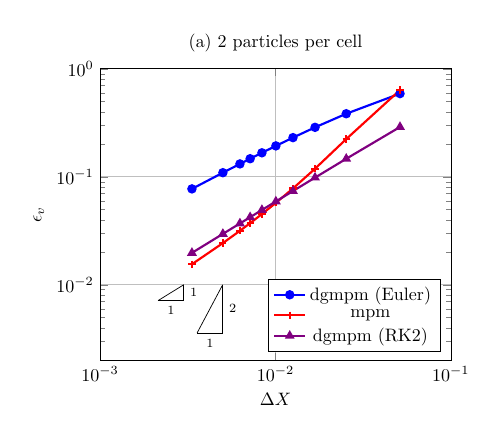
\begin{tikzpicture}[scale=0.65]
\begin{loglogaxis}[xlabel=$\Delta X$,ylabel=$\epsilon_v$,ymajorgrids=true,xmajorgrids=true,legend pos=south east,title={(a) 2 particles per cell},xtick={0.1,0.01,0.001},xmin=0.001,xmax=0.1,ymin=0.002,ymax=1.]
\addplot[Blue,very thick,mark=*] coordinates {(0.05128205128205128,0.5892536463713801) (0.025316455696202535,0.38365022009201677) (0.01680672268907563,0.2869412166132242) (0.012578616352201259,0.23042992589433486) (0.010050251256281405,0.19320644118388566) (0.008368200836820083,0.1667585144216507) (0.007168458781362007,0.14695767904169704) (0.006269592476489028,0.13155393217242617) (0.005012531328320802,0.10909713160359168) (0.00333889816360601,0.07724729297813987) };
\addplot[Red,very thick,mark=+] coordinates {(0.05128205128205128,0.635815700712952) (0.025316455696202535,0.2234315557871451) (0.01680672268907563,0.1187663338566914) (0.012578616352201259,0.07796811784294516) (0.010050251256281405,0.057330072742400845) (0.008368200836820083,0.04514285954655251) (0.007168458781362007,0.03718100625696033) (0.006269592476489028,0.03159983501497456) (0.005012531328320802,0.02431876909087104) (0.00333889816360601,0.015492293355593201) };
\addplot[Purple,very thick,mark=triangle*] coordinates {(0.05128205128205128,0.28917389811427335) (0.025316455696202535,0.146795101418884) (0.01680672268907563,0.09821148280234744) (0.012578616352201259,0.07377182111730703) (0.010050251256281405,0.0590675963901161) (0.008368200836820083,0.04924943612717912) (0.007168458781362007,0.04222940622094088) (0.006269592476489028,0.036960694946397976) (0.005012531328320802,0.02957940251610272) (0.00333889816360601,0.019728868588375394) };
\legend{dgmpm (Euler),mpm,dgmpm (RK2)}
\draw (axis cs:0.003,0.01) -- (axis cs:0.003/1.4,0.01/1.4) ;
\draw (axis cs:0.003,0.01) -- (axis cs:0.003,0.01/1.4) node [midway,right] {\scriptsize 1};
\draw (axis cs:0.003,0.01/1.4) -- (axis cs:0.003/1.4,0.01/1.4) node [midway,below] {\scriptsize 1};
%% second order 
\draw (axis cs:0.005,0.01) -- (axis cs:0.005/1.4,0.01/2.8) ;
\draw (axis cs:0.005,0.01) -- (axis cs:0.005,0.01/2.8) node [midway,right] {\scriptsize 2};
\draw (axis cs:0.005,0.01/2.8) -- (axis cs:0.005/1.4,0.01/2.8) node [midway,below] {\scriptsize 1};
\end{loglogaxis}
\end{tikzpicture}

%%% Local Variables:
%%% mode: latex
%%% TeX-master: "../../mainManuscript.tex"
%%% End:
}
  {\definecolor{Purple}{RGB}{120,28,129}
\definecolor{Blue}{RGB}{63,96,174}
\definecolor{Duck}{RGB}{83,158,182}
\definecolor{Green}{RGB}{109,179,136}
\definecolor{Yellow}{RGB}{202,184,67}
\definecolor{Orange}{RGB}{231,133,50}
\definecolor{Red}{RGB}{217,33,32}
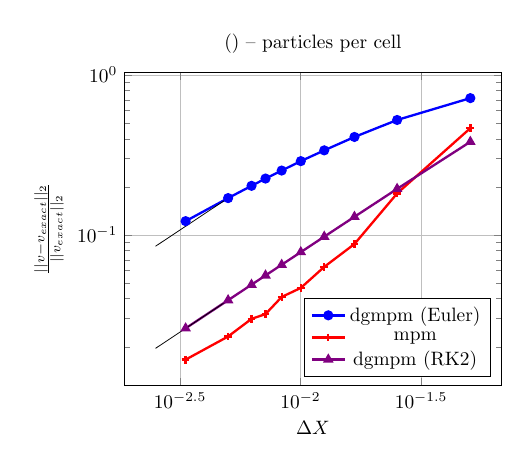
\begin{tikzpicture}[scale=0.7]
\begin{loglogaxis}[xlabel=$\Delta X$,ylabel=$\frac{||v- v_{exact}||_2}{||v_{exact}||_2}$,ymajorgrids=true,xmajorgrids=true,legend pos=south east,title={() -- particles per cell}]
\addplot[Blue,very thick,mark=*] coordinates {(0.05063291139240507,0.7174221864294394) (0.02515723270440252,0.5237236302081432) (0.016736401673640166,0.4101568719062216) (0.012539184952978056,0.3382439911559517) (0.010025062656641603,0.2896270216843742) (0.008350730688935281,0.25286527819449833) (0.007155635062611806,0.22536895047570651) (0.00625978090766823,0.2029809636649474) (0.005006257822277847,0.1701404944130945) (0.003336113427856547,0.12210227819385817) };
\addplot[Red,very thick,mark=+] coordinates {(0.05063291139240507,0.4653787886720093) (0.02515723270440252,0.1819539127995734) (0.016736401673640166,0.08783874642012299) (0.012539184952978056,0.06320726759321203) (0.010025062656641603,0.046691706110167805) (0.008350730688935281,0.04098750239541997) (0.007155635062611806,0.03203505037423235) (0.00625978090766823,0.029906266183517122) (0.005006257822277847,0.02320647763349648) (0.003336113427856547,0.016629938499808216) };
\addplot[Purple,very thick,mark=triangle*] coordinates {(0.05063291139240507,0.38264834434819694) (0.02515723270440252,0.19428758292892198) (0.016736401673640166,0.12998482541796058) (0.012539184952978056,0.09763321880245852) (0.010025062656641603,0.078168883492807) (0.008350730688935281,0.06517289166505665) (0.007155635062611806,0.0558811340004746) (0.00625978090766823,0.04890774174042707) (0.005006257822277847,0.03913878524154382) (0.003336113427856547,0.026103030284649532) };
\legend{dgmpm (Euler),mpm,dgmpm (RK2)}\addplot[black] coordinates {(0.005006257822277847,0.03913878524154382) (0.0025031289111389233,0.01956939262077191)};\addplot[black] coordinates {(0.005006257822277847,0.1701404944130945) (0.0025031289111389233,0.08507024720654725)};
\end{loglogaxis}
\end{tikzpicture}
}
  \caption{Velocity convergence curves}
  \label{fig:convergence_4ppc}
\end{figure}

Therefore one can imagine to adapt the material points discretization so that a givan order of accuracy is achieved. Such an adaption of the particles positions must be however made by keeping fixed boundary material points.

\subsection{Two-dimensional stability analysis}
\subsubsection*{Model equation - Space discretization}
We now focus on the scalar linear advection equation for an arbitrary quantity $q=\rho \bar{q}$ moving at constant speeds $a,b \in \Rbb^{+*}$ in $X$ and $Y$ directions respectively in a homogeneous two-dimensional medium:
\begin{equation}
  \label{eq:2D_model_equation}
  \drond{\bar{q}}{t} + a\drond{\bar{q}}{X} + b\drond{\bar{q}}{Y}= 0
\end{equation}
Note that the flux functions are in that case $\bar{f}^X = a\bar{q}$ and $\bar{f}^Y = b\bar{q}$. The physical domain $[0,l]\times[0,h]$ is discretized with $N_p$ material points arbitrarily distributed in a Cartesian grid made of $E$ four-nodes bilinear elements with constant size $\Delta X \times \Delta Y$. Horizontal and vertical edges lengths are distinguished here in spite of the Cartesian nature of the grid in order to easily extend the following study to rectilinear grids. Again, there is no empty cell inside the physical domain so that no hole is generated, and periodic boundary conditions are considered to simplify the analysis.

\subsubsection*{Two-dimensional scheme equation}
One can imagine to combine the DGMPM discretization with a multi-stages time integration as proposed for one-dimensional problems The analysis of the DGMPM scheme for two-dimensional problems carried out here however only consider the Euler time discretization. As we shall see, the use of the CTU method (see section \ref{subsec:interface_fluxes}) introduces second-order corrections in time to the orginial DCU approach. Therefore, the updated solution at material point $\alpha$ is obtained by interpolation of nodal solutions satisfiying equation \eqref{eq:2D_model_equation}, discretized as:
\begin{equation}
  \bar{q}_i^{n+1} = \bar{q}_i^n + \frac{\Delta t}{M^L_i} \(K_{ij}^X a\bar{q}_j^n + K_{ij}^Y b\bar{q}_j^n - \hat{f}_i^{*}\) \label{eq:discrete2D}
\end{equation}
so that:
\begin{equation}
  \label{eq:2D_updatedMP}
  \bar{Q}^{n+1}_\alpha = \sum_{i=1}^{4E}S_{_\alpha} \bar{q}_i^{n+1}
\end{equation}
\begin{figure}[ht]
  \centering
  \begin{tikzpicture}
  \draw[thick,->] (-1.5,0.)--(1.5,0.) node [right] {$\xi$};
  \draw[thick,->] (0.,-1.5)--(0.,1.5) node [above] {$\eta$};
  \draw (-1.,-1.0) rectangle (1.,1.);
  \node[above right] at (0.,1.) {$1$};\node[above right] at (0.,-1.) {-$1$};
  \node[above right] at (-1,0.) {-$1$};\node[above right] at (1.,.) {$1$};
  \draw[thick,->] (-.25+5.,0.)--(1.5+5.,0.) node [right] {$X$};
  \draw[thick,->] (0.+5.,-.25)--(0.+5.,1.5) node [above] {$Y$};
  % origin at (+5.,0.)
  \draw (6.,1.) node [below] {$X_1$}-- (8.,1.5) node [below] {$X_2$}-- (9.,4.) node [above] {$X_3$}-- (6.5,3.5) node [above] {$X_4$}-- (6.,1.);
  \fill[black] (8.,3.25) circle (0.05) node [above] {$\vect{X}$};
  \fill[black] (.5,.5) circle (0.05) node [above] {$\vect{\xi}$};
  \draw[->] (8.,3.25) .. controls (6.,3.25) and (1.5,1.5) .. (.5,.5);
\end{tikzpicture}
  
  \caption{Parent and current configuration of a four-nodes bilinear element}
  \label{fig:2Dparent}
\end{figure}
The lumped mass matrix in equation \eqref{eq:discrete2D} has the same expression as in the one-dimensional case, that depends on the shape functions of the four-nodes bilinear element: $M_i^L=\sum_\mu m_\mu S_{i\mu}$. Next, the position of the $i$th node of cell $C$, denoted by $\vect{X}_i^C=\matrice{X^C_i \\ Y_i^C}$, maps to the parent coordinates $(\xi,\eta)$ in the domain $\[-1,1\]\times\[-1,1\]$ according to:
\begin{equation}
  \label{eq:parentCoordinates}
  \begin{aligned}
      &\xi = 2\frac{X-X^C_1}{\Delta X} -1 \quad ; \quad d\xi = 2\frac{dX}{\Delta X} \\
      &\eta = 2\frac{Y-Y^C_1}{\Delta Y} -1 \quad ; \quad d\eta = 2\frac{dY}{\Delta Y} 
  \end{aligned}
\end{equation}

Therefore, the pseudo-stiffness matrices read:
\begin{equation}
  \begin{aligned}
    & K_{ij}^X = \sum_\beta \drond{S_{i\beta}}{X}m_\beta S_{j\beta}=\frac{2}{\Delta X}\sum_\beta\drond{S_{i\beta}}{\xi}m_\beta S_{j\beta} \\
    &K_{ij}^Y = \sum_\beta\drond{S_{i\beta}}{Y}m_\beta S_{j\beta}=\frac{2}{\Delta Y}\sum_\beta\drond{S_{i\beta}}{\eta}m_\beta S_{j\beta} \\
  \end{aligned}
\end{equation}
and subsequently, by writing $\drond{(\bullet)}{\xi}=\partial_\xi(\bullet)$:
\begin{equation}
  \label{eq:2Dpseudo_stiffness}
  \begin{aligned}
    & \frac{K_{ij}^X}{M_i^L}  =  \frac{2}{\Delta X} \frac{\sum_\lambda\partial_\xi S_{i\lambda}  S_{j\lambda}}{\sum_\gamma  S_{i\gamma}} \\
    & \frac{K_{ij}^Y}{M_i^L} = \frac{2}{\Delta Y} \frac{\sum_\lambda\partial_\eta S_{i\lambda} S_{j\lambda}}{\sum_\gamma S_{i\gamma}}
  \end{aligned}
\end{equation}
The nodal solutions at time $n$ being given by the convective phase $\bar{q}^{C,n}_i=\frac{\sum_\beta S_{i\beta}\bar{Q}^n_\beta}{\sum_\gamma S_{i\gamma}}$, the volume fluxes of the discrete form can be rewritten as:
\begin{equation}
  \label{eq:2Dvolume_fluxes}
  \begin{aligned}
    & a\frac{K_{ij}^X}{M_i^L}\bar{q}^n_j  = \sum_\beta \bar{Q}^n_\beta \frac{2}{\Delta X} \frac{a\sum_\lambda\partial_\xi S_{i\lambda}  \sum_j S_{j\lambda} S_{j\beta}}{\sum_\gamma  S_{i\gamma}\sum_\mu S_{j\mu}}\\
    & b\frac{K_{ij}^Y}{M_i^L}\bar{q}^n_j = \sum_\beta \bar{Q}^n_\beta\frac{2}{\Delta Y}  \frac{b \sum_\lambda\partial_\eta S_{i\lambda}  \sum_j S_{j\lambda} S_{j\beta}}{\sum_\gamma  S_{i\gamma}\sum_\mu S_{j\mu}}
  \end{aligned}
\end{equation}
Moreover, nodal interface flux $\hat{f}_i^{*}$ results from the integration of Godunov's flux along the edges it belongs to, according to the weak form \eqref{eq:DGMPM_semi_discrete}.
Referring to a quantity defined at an interface by means of parenthesis superscripts, the Godunov's flux corresponding to equation \eqref{eq:2D_model_equation} at interface $(i)$ is:
\begin{equation}
  \label{eq:2d_Godunov_fluxes}
  f^{(i)}= c_n q^{(i)}_U = \underbrace{c_nq^{(i)}_D}_{f_N(q^{(i)}_D)} - \underbrace{c_n (q^{(i)}_D -q^{(i)}_U)}_{A^{+}_{U/D}} 
\end{equation}
where $c_n$ is the speed in the direction normal to the interface (\textit{i.e. b for horizontal and a for vertical edges}). Equation \eqref{eq:2d_Godunov_fluxes} further involves state vectors $q^{(i)}_U$ and $q^{(i)}_D$ obtained by averaging nodal values connected to interface $(i)$ on Upwind and Downwind sides respectively, and the right-going fluctuation $A_{U/D}^+$.
The CTU is adopted by accounting for transverse corrections based on those fluctuations according to equation \eqref{eq:transverse_fluctuations}:
\begin{equation}
  \label{eq:2D_transverse_corrections}
  B^+A^+_{U/D}=c_t c_n (q^{(i)}_D -q^{(i)}_U)
\end{equation}
with $c_t$ the speed in the direction tangent to the edge.
\begin{figure}[h!]
  \centering
  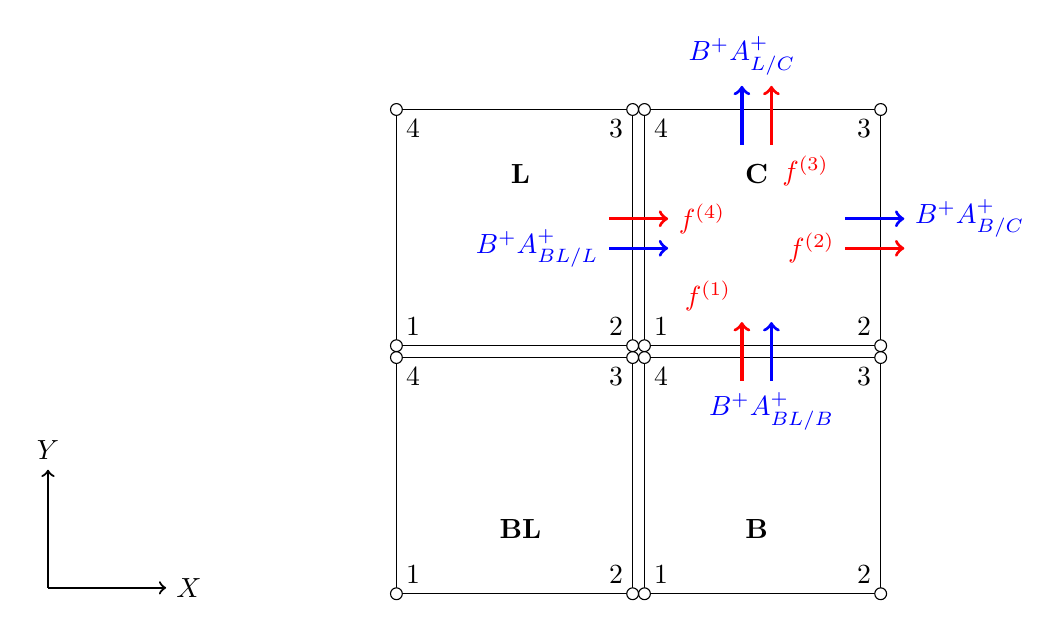
\begin{tikzpicture}[scale=1.5]
  \draw[thick,->] (-3,0.)-- (-2,0.) node[right] {$X$};
  \draw[thick,->] (-3,0.)-- (-3,1.) node[above] {$Y$};

  %% Cells
  \draw (0-0.05,0-0.05) rectangle (2.-0.05,2-0.05);
  \draw (0-0.05,2+0.05) rectangle (2.-0.05,4+0.05);
  \draw (2+0.05,0-0.05) rectangle (4.+0.05,2-0.05);
  \draw (2+0.05,2+0.05) rectangle (4.+0.05,4+0.05);
  %%%%%%%%%%%%%%%%%%%%%
  
  %% Nodes
  \fill[white] (0-0.05,0-0.05) circle (0.05);\fill[white] (2-0.05,2-0.05) circle (0.05);
  \fill[white] (0-0.05,2+0.05) circle (0.05);\fill[white] (2.-0.05,4+0.05) circle (0.05);
  \fill[white] (2+0.05,0-0.05) circle (0.05);\fill[white] (4.+0.05,2-0.05) circle (0.05);
  \fill[white] (2+0.05,2+0.05) circle (0.05);\fill[white] (4.+0.05,4+0.05) circle (0.05);
  \fill[white] (2-0.05,0-0.05) circle (0.05);\fill[white] (4.+0.05,0-0.05) circle (0.05);
  \fill[white] (0-0.05,2-0.05) circle (0.05);\fill[white] (2.+0.05,2-0.05) circle (0.05);
  \fill[white] (2-0.05,2+0.05) circle (0.05);\fill[white] (4.+0.05,2.+0.05) circle (0.05);
  \fill[white] (-0.05,4+0.05) circle (0.05);\fill[white] (2.+0.05,4+0.05) circle (0.05);

  \draw (0-0.05,0-0.05) circle (0.05) node[above right] {$1$};\draw (2-0.05,2-0.05) circle (0.05) node[below left] {$3$};
  \draw (0-0.05,2+0.05) circle (0.05) node[above right] {$1$};\draw (2.-0.05,4+0.05) circle (0.05) node[below left] {$3$};
  \draw (2+0.05,0-0.05) circle (0.05) node[above right] {$1$};\draw (4.+0.05,2-0.05) circle (0.05) node[below left] {$3$};
  \draw (2+0.05,2+0.05) circle (0.05) node[above right] {$1$};\draw (4.+0.05,4+0.05) circle (0.05) node[below left] {$3$};
  \draw (2-0.05,0-0.05) circle (0.05) node[above left] {$2$};\draw (4.+0.05,0-0.05) circle (0.05) node[above left] {$2$};
  \draw (0-0.05,2-0.05) circle (0.05) node[below right] {$4$};\draw (2.+0.05,2-0.05) circle (0.05) node[below right] {$4$};
  \draw (2-0.05,2+0.05) circle (0.05) node[above left] {$2$};\draw (4.+0.05,2.+0.05) circle (0.05) node[above left] {$2$};
  \draw (-0.05,4+0.05) circle (0.05) node[below right] {$4$};\draw (2.+0.05,4+0.05) circle (0.05) node[below right] {$4$};
  %%%%%%%%%%%%%%%%%%%%%%%

  %% Cells names
  \node at (3,3.5) {$\textbf{C}$};
  \node at (1,0.5) {$\textbf{BL}$};
  \node at (3,0.5) {$\textbf{B}$};
  \node at (1,3.5) {$\textbf{L}$};

  %% Transverse corrections
  \draw[->, very thick,Blue] (2.875,3.75) -- (2.875,4.25) node [above] {$B^+A^+_{L/C}$}; % Top
  \draw[->, very thick,Blue] (3.75,3.125) -- (4.25,3.125) node [right] {$B^+A^+_{B/C}$}; % Right
  \draw[<-, very thick,Blue] (3.125,2.25) -- (3.125,1.75) node [below] {$B^+A^+_{BL/B}$}; % Bottom
  \draw[<-, very thick,Blue] (2.25,2.875) -- (1.75,2.875) node [left] {$B^+A^+_{BL/L}$}; % Left

  %% Normal fluxes
  \draw[->, very thick,Red] (3.125,3.75) node [below right] {$f^{(3)}$} -- (3.125,4.25) ; % Top
  \draw[->, very thick,Red] (3.75,2.875) node [left] {$f^{(2)}$}-- (4.25,2.875) ; % Right
  \draw[<-, very thick,Red] (2.875,2.25) node [above left] {$f^{(1)}$}-- (2.875,1.75); % Bottom
  \draw[<-, very thick,Red] (2.25,3.125) node [right] {$f^{(4)}$} -- (1.75,3.125); % Left

  % %% Edges numbers
  % \node[above] at (1,-0.1) {$(1)$};
  % \node[left] at (2,1.) {$(2)$};
  % \node[below] at (1,1.95) {$(3)$};
  % \node[right] at (-0.1,1.) {$(4)$};
\end{tikzpicture}


%%% Local Variables:
%%% mode: latex
%%% TeX-master: "../../mainManuscript"
%%% End:

  \caption{Two-dimensional patch of cells of constant size $\Delta X \times \Delta Y$.}\label{fig:2Dmesh}
\end{figure}
Figure \ref{fig:2Dmesh} shows transverse corrections in the cell $C$ which are based on fluctuations coming from Bottom ($B$), Left ($L$), Bottom Left ($BL$) neighor elements of that cell. The use of the numbering of interfaces and nodes adopted in figure \ref{fig:2Dmesh} allows the specialization of the above formula to intercell fluxes of cell $C$:
\begin{align}
  & f^{(1)} = b \frac{q_3^{B,n} + q_4^{B,n}}{2} - a b \frac{\Delta t}{2\Delta Y}\(\frac{q_1^{B,n}+q_4^{B,n}}{2}-\frac{q_2^{BL,n}+q_3^{BL,n}}{2}\) \\
  & f^{(2)} = a \frac{q_2^{C,n} + q_3^{C,n}}{2} - a b \frac{\Delta t}{2\Delta X}\(\frac{q_1^{C,n}+q_2^{C,n}}{2}-\frac{q_3^{B,n}+q_4^{B,n}}{2}\) \\
  & f^{(3)} = b \frac{q_3^{C,n} + q_4^{C,n}}{2} - a b \frac{\Delta t}{2\Delta Y}\(\frac{q_1^{C,n}+q_4^{C,n}}{2}-\frac{q_2^{L,n}+q_3^{L,n}}{2}\) \\
  & f^{(4)} = a \frac{q_3^{L,n} + q_4^{L,n}}{2} - a b \frac{\Delta t}{2\Delta X}\(\frac{q_1^{L,n}+q_2^{L,n}}{2}-\frac{q_3^{BL,n}+q_4^{BL,n}}{2}\)
\end{align}
where $q^{C,n}_i= \rho \bar{q}^{C,n}_i$ is the value at time step $n$ and node $i$ of cell $C$ in which the uniform mass density is defined as $\rho = \frac{N_p^{C} m^C}{\Delta X \Delta Y}$ with $N_p^C$, the total number of particles in that element, and $m^C$ the mass they carry. Thus, introduction of the convective phase yields the following expressions for interface fluxes:
\begin{align}
  & f^{(1)} = \sum_{\beta=1}^{N_p}\bar{q}_\beta^n\frac{b N^C_p m^C }{2\Delta X \Delta Y} \[  \(\frac{S_{3\beta}^{B} }{\sum_\gamma S_{3\gamma}^{B}} + \frac{S_{4\beta}^{B}}{\sum_\gamma S_{4\gamma}^{B}}\) - a  \frac{\Delta t}{2\Delta Y}\(\frac{S_{1\beta}^{B}}{\sum_\gamma S_{1\gamma}^B} + \frac{S_{4\beta}^{B}}{\sum_\gamma S_{4\gamma}^{B} }-\frac{S_{2\beta}^{BL}}{\sum_\gamma S_{2\gamma}^{BL}} - \frac{S_{3\beta}^{BL}}{\sum_\gamma S_{3\gamma}^{BL}}\) \]\\
  & f^{(2)} = \sum_{\beta=1}^{N_p} \bar{q}_\beta^n\frac{a N^C_p m^C }{2\Delta X \Delta Y} \[  \(\frac{S_{2\beta}^{C}}{\sum_\gamma S_{2\gamma}^{C}} + \frac{S_{3\beta}^{C}}{\sum_\gamma S_{3\gamma}^{C}} \)- b \frac{\Delta t}{2\Delta X}\(\frac{S_{1\beta}^{C}}{\sum_\gamma S_{1\gamma}^{C}} + \frac{S_{2\beta}^{C}}{\sum_\gamma S_{2\gamma}^{C}}-\frac{S_{3\beta}^{B}}{\sum_\gamma S_{3\gamma}^{B}} -\frac{S_{4\beta}^{B}}{\sum_\gamma S_{4\gamma}^{B}}\) \]\\
  & f^{(3)} =\sum_{\beta=1}^{N_p}\bar{q}_\beta^n\frac{b N^C_p m^C}{2\Delta X \Delta Y} \[  \(\frac{S_{3\beta}^{C}}{\sum_\gamma S_{3\gamma}^{C}} + \frac{ S_{4\beta}^{C}}{\sum_\gamma S_{4\gamma}^{C}}\) - a  \frac{\Delta t}{2\Delta Y}\(\frac{S_{1\beta}^{C}}{\sum_\gamma S_{1\gamma}^{C}} + \frac{S_{4\beta}^{C}}{\sum_\gamma S_{4\gamma}^{C}}-\frac{S_{2\beta}^{L}}{\sum_\gamma S_{2\gamma}^{L}} - \frac{S_{3\beta}^{L}}{\sum_\gamma S_{3\gamma}^{L}}\) \]\\
  & f^{(4)} = \sum_{\beta=1}^{N_p}\bar{q}_\beta^n\frac{a N^C_p m^C }{2\Delta X \Delta Y}  \[  \(\frac{S_{3\beta}^{L}}{\sum_\gamma S_{3\gamma}^{L}} + \frac{ S_{4\beta}^{L}}{\sum_\gamma S_{4\gamma}^{L}}\) - b \frac{\Delta t}{2\Delta X}\(\frac{S_{1\beta}^{L}}{\sum_\gamma S_{1\gamma}^{L}} + \frac{S_{2\beta}^{L}}{\sum_\gamma S_{2\gamma}^{L}}-\frac{S_{3\beta}^{BL}}{\sum_\gamma S_{3\gamma}^{BL}} - \frac{S_{4\beta}^{BL}}{\sum_\gamma S_{4\gamma}^{L}}\)\]
\end{align}
written for simplicity:
\begin{equation}
  \label{eq:interface_flux_mapped}
  f^{(i)}=\sum^{N_p}_\beta \bar{Q}_\beta^n \frac{c_n N^C_p m^C}{2\Delta X \Delta Y}\[ \phi_\beta^{(i)} + \phi_\beta^{(i),T} \]
\end{equation}
In the latter expressions, $\phi^{(i)}$ is devoted to normal contributions while $\phi^{(i),T}$ stands for transverse corrections at interface $(i)$. Numerical fluxes considered above are based on normal vectors oriented in the direction of the stream (see figure \ref{fig:2Dmesh}). Nodal interface fluxes on the other hand, as defined in the semi-discrete system:
%Fluxes contribute to nodes through the boundary integrals of the discrete form:
\begin{equation}
  \hat{f}_i^{*} = \int_{\Gamma} S_i(\vect{X}) f^*_N  \: d\Gamma
\end{equation}
are based on the outgoing flux to an element so that $f^{(1)}$ and $f^{(4)}$ must be counted negatively. The integral then reads for cell $C$:
\begin{equation}
  \hat{f}_i^{*} =  -\int_{X^C_1}^{X_2^C} S_i(X,Y^C_{1}) f^{(1)}  dX + \int_{Y^C_2}^{Y_3^C} S_i(X^C_{2},Y) f^{(2)}  dY +\int_{X^C_2}^{X_3^C} S_i(X,Y^C_{3}) f^{(3)}  dX -\int_{Y^C_1}^{Y_4^C} S_i(X^C_{1},Y) f^{(4)}  dY 
\end{equation}
which can be computed analytically by using parent coordinates \eqref{eq:parentCoordinates}:
\begin{subequations}
  \begin{alignat}{4}
    &\hat{f}_1^{*} = -&\frac{1}{2}\[\Delta X f^{(1)} + \Delta Y f^{(4)}\] \quad;\quad &\hat{f}_2^{*} = -&\frac{1}{2}\[\Delta X f^{(1)} - \Delta Y f^{(2)}\]\\
    &\hat{f}_3^{*} =  &\frac{1}{2}\[\Delta X f^{(3)} + \Delta Y f^{(2)}\] \quad;\quad &\hat{f}_4^{*} = &\frac{1}{2}\[\Delta X f^{(3)} - \Delta Y f^{(4)}\]
  \end{alignat}
\end{subequations}
A condensed way of writing the fluxes can be adopted by introducing the middle point of edges, with coordinates denoted by $\vect{X}^{(i)}_{1/2}$, at which the shape functions are:
\begin{equation*}
  S_i(\vect{X}^{(j)}_{1/2}) =
  \left\lbrace
  \begin{aligned}
    & \frac{1}{2} \quad \text{if node i belongs to edge (j)} \\
    & 0 \quad \text{otherwise.}
  \end{aligned}
  \right.
\end{equation*}
In addition, components of the outward normal vector to edges $N^{(i)}_X$ and $N^{(i)}_Y$ allows to take into account different signs of intercell fluxes in the Cartesian grid. One thus writes:
\begin{equation}
  \hat{f}_i^{*}= \frac{1}{2}\sum_j^{\text{edges}} 2S_{i}(\vect{X}^{(j)}_{1/2})\(\Delta Y N^{(j)}_X + \Delta X N^{(j)}_Y\) f^{(j)}
\end{equation}
which, combined to equation \eqref{eq:interface_flux_mapped} leads to:
\begin{equation}
  \hat{f}_i^{*}= \sum^{N_p}_\beta \bar{Q}_\beta^n \sum_j^{\text{edges}} S_{i}(\vect{X}^{(j)}_{1/2})\(a\Delta Y N^{(j)}_X + b\Delta X N^{(j)}_Y\)  \frac{ N^C_p m^C}{2\Delta X\Delta Y}\[ \phi_\beta^{(i)} + \phi_\beta^{(i),T} \]
\end{equation}
These terms are divided by the lumped mass matrix in the discrete form:
\begin{equation}
  \label{eq:nodal_fluxes}
  \frac{\hat{f}_i^{*}}{M_i^L}=\sum_\beta \frac{\bar{Q}_\beta^n}{\sum_\mu S_{i\mu}}   \sum_{j=1}^{\text{edges}}\frac{1}{2} S_{i}(\vect{X}^{(j)}_{1/2}) N^C_p m^C \(\frac{aN^{(j)}_X}{\Delta X}  + \frac{bN^{(j)}_Y}{\Delta Y} \) \[\phi_\beta^{(j)} + \phi_\beta^{(j),T}\] 
\end{equation}

At last, gathering the mapping of updated nodal quantities to the particle \eqref{eq:2D_updatedMP}, expressions of volume fluxes \eqref{eq:2Dvolume_fluxes} and intercell ones \eqref{eq:nodal_fluxes}, the updated value at material point $\alpha$ contained in cell $C$ reads:
\begin{equation}
  \label{eq:2Dscheme_equation}
  \begin{split}
    \bar{Q}_\alpha^{n+1}=  \sum_{\beta=1}^{N_p}\bar{Q}_\beta^n\sum_{i=1}^{4E}\frac{S_{i\alpha}}{\sum_\mu S_{i\mu}}  \left\lbrace \vphantom{\sum_{j=1}^{\text{edges}} } \right.& S_{i\beta} +  2  \sum_{j=1}^{4E} \frac{ S_{j\beta}}{\sum_\gamma S_{j\gamma}}\sum_{\lambda=1}^{N_p}S_{j\lambda}\[ a\frac{\Delta t}{\Delta X}\partial_\xi S_{i\lambda}  + b\frac{\Delta t}{\Delta Y} \partial_\eta S_{i\lambda} \] \\ - & \frac{1}{2}\left.\sum_{k=1}^{\text{edges}} S_{i}(\vect{X}^{(k)}_{1/2}) N_p^C \(a\frac{\Delta t}{\Delta X}N^{(j)}_X  + b\frac{\Delta t}{\Delta Y}N^{(j)}_Y \)\[\phi_\beta^{(k)} + \phi_\beta^{(k),T}\] \right\rbrace
  \end{split}
\end{equation}
Recall that in the two-dimensional scheme equation \eqref{eq:2Dscheme_equation}, transverse contributions $\phi_\beta^{(j),T}$ depend on $\Delta t$, providing thus second order corrections in time. Equation \eqref{eq:2Dscheme_equation} can also be rewritten as:
\begin{equation}
  \label{eq:2Dscheme_D_alphabeta}
  \bar{Q}_\alpha^{n+1}= \sum_{\beta=1}^{N_p}\bar{Q}_\beta^n D_{\alpha\beta}
\end{equation}

\subsubsection*{The von Neumann linear stability analysis}
Analogously to the one-dimensonal case, the solution at a material point can be expanded into a discrete Fourier basis over the domain $\[-l,l\]\times\[-h,h\]$. We consider here a structured discretization made of $N_p=N_p^X\times N_p^Y$ material points so that one can denote the solution at particles by $\bar{Q}_{\alpha\beta}$, where $\alpha$ and $\beta$ are the row and column of material points indices. For one arbitrary Fourier mode, one has \cite{Leveque}:
\begin{equation}
\bar{Q}^{n}_{\alpha \beta} = A_{jq}^n e^{i (\alpha k_j + \beta k_q)\Delta X}
\end{equation}
where $k_j$ and $k_q$ are wave numbers. Then, the amplification factor reads:
\begin{equation}
\frac{A_{jq}^{n+1}}{A_{jq}^n} =  \sum_{\gamma=1}^{N_p^X}\sum_{\mu=1}^{N_p^Y} e^{i ([\alpha-\gamma]k_j + [\beta-\mu]k_q)\Delta X}D_{\alpha\beta,\gamma\mu}
\end{equation}
with $i=\sqrt{-1}$. The requirement that the absolute value of the amplification factor is lower than or equal one leads to the following stability condition which is similar to that of one-dimensional problems:
\begin{equation}
\abs{\frac{A_{jq}^{n+1}}{A_{jq}^n}} = \abs{\sum_{\gamma=1}^{N_p^X}\sum_{\mu=1}^{N_p^Y} e^{i ([\alpha-\gamma]k_j + [\beta-\mu]k_q)\Delta X}D_{\alpha\beta,\gamma\mu}} \leq 1 \Leftrightarrow  \sum_{\gamma=1}^{N_p^X}\sum_{\mu=1}^{N_p^Y} \abs{D_{\alpha\beta,\gamma\mu}} \leq 1
\end{equation}
or more simply:
\begin{equation}
\sum_{\beta=1}^{N_p} \abs{D_{\alpha\beta}} \leq 1 \quad \forall \alpha=1,...,N_p
\end{equation}

Again, the convective phase leads for the single particle-per-cell discretization to a piece-wise constant reconstruction of the field on the computational grid thus providing the first order upwind method. This method is known to be bounded by the stability requirements \cite[p.449]{Leveque}:
\begin{subequations}
  \label{eq:2DCFL}
  \begin{alignat}{2}
    & \abs{a}\frac{\Delta t}{\Delta X} + \abs{b} \frac{\Delta t}{\Delta Y} \leq 1 \qquad &\text{for DCU} \\
    & \max \( \abs{a} \frac{\Delta t}{\Delta X}  , \abs{b} \frac{\Delta t}{\Delta Y}\) \leq 1 \qquad &\text{for CTU}
  \end{alignat}
\end{subequations}

% \begin{table}[h]
%   \centering
%   \begin{tabular}[ht]{M{2cm}M{8cm}M{1cm}M{1cm}}
  %\setlength\extrarowheight{2.5pt}
  \hline
   Particles & Position of particles in cell $c$ & DCU & CTU \\
  \hline
  \hline
  2 & 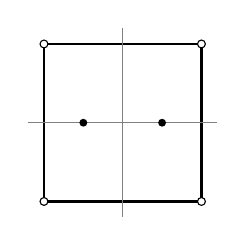
\begin{tikzpicture}[scale=1.]
    \draw[thick] (-1.,-1.) rectangle (1.,1.);
    \draw[black!50] (-1.2,0.) -- (1.2,0.0);\draw[black!50] (.0,-1.2) -- (0.,1.2);
    %% nodes
    \fill[white] (-1,-1) circle (0.05);\draw (-1,-1) circle (0.05);
    \fill[white] (1.,-1) circle (0.05);\draw (1,-1) circle (0.05);
    \fill[white] (1,1) circle (0.05);\draw (1,1) circle (0.05);
    \fill[white] (-1.,1) circle (0.05);\draw (-1,1) circle (0.05);
    %% particles
    \fill[black] (-0.5,0.) circle (0.05);
    \fill[black] (0.5,0.) circle (0.05);
  \end{tikzpicture} 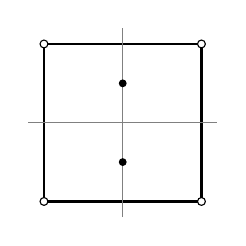
\begin{tikzpicture}[scale=1.]
    \draw[thick] (-1.,-1.) rectangle (1.,1.);
    \draw[black!50] (-1.2,0.) -- (1.2,0.0);\draw[black!50] (.0,-1.2) -- (0.,1.2);
    %% nodes
    \fill[white] (-1,-1) circle (0.05);\draw (-1,-1) circle (0.05);
    \fill[white] (1.,-1) circle (0.05);\draw (1,-1) circle (0.05);
    \fill[white] (1,1) circle (0.05);\draw (1,1) circle (0.05);
    \fill[white] (-1.,1) circle (0.05);\draw (-1,1) circle (0.05);
    %% particles
    \fill[black] (0.,-0.5) circle (0.05);
    \fill[black] (0.,0.5) circle (0.05);
  \end{tikzpicture} &  0.27 & 0.28\\ %%% SOLUTION
  \hline
  2 & 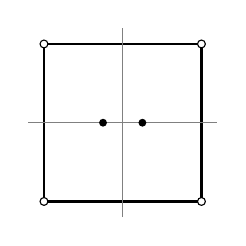
\begin{tikzpicture}[scale=1.]
    \draw[thick] (-1.,-1.) rectangle (1.,1.);
    \draw[black!50] (-1.2,0.) -- (1.2,0.0);\draw[black!50] (.0,-1.2) -- (0.,1.2);
    %% nodes
    \fill[white] (-1,-1) circle (0.05);\draw (-1,-1) circle (0.05);
    \fill[white] (1.,-1) circle (0.05);\draw (1,-1) circle (0.05);
    \fill[white] (1,1) circle (0.05);\draw (1,1) circle (0.05);
    \fill[white] (-1.,1) circle (0.05);\draw (-1,1) circle (0.05);
    %% particles
    \fill[black] (-0.25,0.) circle (0.05);
    \fill[black] (0.25,0.) circle (0.05);
  \end{tikzpicture} 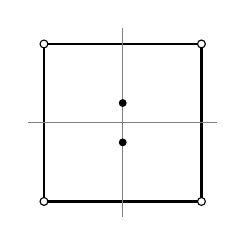
\begin{tikzpicture}[scale=1.]
    \draw[thick] (-1.,-1.) rectangle (1.,1.);
    \draw[black!50] (-1.2,0.) -- (1.2,0.0);\draw[black!50] (.0,-1.2) -- (0.,1.2);
    %% nodes
    \fill[white] (-1,-1) circle (0.05);\draw (-1,-1) circle (0.05);
    \fill[white] (1.,-1) circle (0.05);\draw (1,-1) circle (0.05);
    \fill[white] (1,1) circle (0.05);\draw (1,1) circle (0.05);
    \fill[white] (-1.,1) circle (0.05);\draw (-1,1) circle (0.05);
    %% particles
    \fill[black] (0.,-0.25) circle (0.05);
    \fill[black] (0.,0.25) circle (0.05);
  \end{tikzpicture} &  0.43 & 1.00\\
  \hline
  4 & 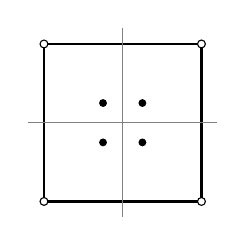
\begin{tikzpicture}[scale=1.]
    \draw[thick] (-1.,-1.) rectangle (1.,1.);
    \draw[black!50] (-1.2,0.) -- (1.2,0.0);\draw[black!50] (.0,-1.2) -- (0.,1.2);
    %% nodes
    \fill[white] (-1,-1) circle (0.05);\draw (-1,-1) circle (0.05);
    \fill[white] (1.,-1) circle (0.05);\draw (1,-1) circle (0.05);
    \fill[white] (1,1) circle (0.05);\draw (1,1) circle (0.05);
    \fill[white] (-1.,1) circle (0.05);\draw (-1,1) circle (0.05);
    %% particles
    \fill[black] (-0.25,-0.25) circle (0.05);
    \fill[black] (0.25,-0.25) circle (0.05);
    \fill[black] (0.25,0.25) circle (0.05);
    \fill[black] (-0.25,0.25) circle (0.05);
  \end{tikzpicture} &  0.43 & 1.00\\%[8pt]
  \hline
  %\begin{minipage}{0.85\textwidth}\lipsum[1]\end{minipage}
\end{tabular}

%%% Local Variables: 
%%% mode: latex
%%% TeX-master: "../../mainManuscript"
%%% End:
%   \caption{DGMPM critical Courant numbers values for Euler or RK2 time integration with respect of the number and positions of material points in a one-dimensional grid. Black circles denote material points while white ones represent grid nodes.}
%   \label{tab:CFL_comparison}
% \end{table}





%%% Local Variables: 
%%% mode: latex
%%% TeX-master: "../mainManuscript"
%%% End:
